\chapter{Programmazione Lineare Intera}
\label{chap:programmazione-lineare-intera}
% Appunti relativi alle pp. 79--105 di RO_Dispense_Festa(2).pdf.
% Capitolo da inserire con \input; non contiene preambolo o document.
% Pacchetti: amsmath, amssymb, amsthm, tikz, caption, needspace.
% Le figure non sono flottanti: sono compatibili con esempi a riquadro.
% Non si usa FloatBarrier e non occorre il pacchetto placeins.
% Librerie TikZ: arrows.meta, calc, positioning.
% Gli ambienti degli enunciati accettano l'argomento obbligatorio {Titolo}.
% I chiarimenti aggiuntivi e le correzioni sono dichiarati nelle osservazioni.

\section{Introduzione}

La \emph{Programmazione Lineare Intera}, abbreviata con \textbf{PLI},
studia problemi di ottimizzazione nei quali la funzione obiettivo e i
vincoli sono lineari, ma le variabili di decisione devono assumere valori
interi. Il vincolo di interezza è essenziale quando le decisioni descrivono
quantità indivisibili, come il numero di mezzi da utilizzare o l'assegnazione
di una persona a un compito.

\begin{definition}{Problema di Programmazione Lineare Intera in forma standard}
Un problema di PLI in forma standard ha la forma
\begin{align*}
(\mathrm{Pli})\qquad \min \quad &z(x)=c^{\mathsf T}x\\
\text{s.a.}\quad &Ax=b,\\
&x\geq0,\qquad x\in\mathbb Z^n,
\end{align*}
dove
\[
A\in\mathbb R^{m\times n},\qquad b\in\mathbb R^m,\qquad c\in\mathbb R^n.
\]
La matrice \(A=(a_{ij})\), con \(i=1,\ldots,m\) e \(j=1,\ldots,n\),
è la \emph{matrice dei coefficienti tecnologici}; \(b\) è il vettore
dei termini noti; \(c\) contiene i coefficienti della funzione obiettivo,
interpretabili come costi nei problemi di minimo e come profitti
nei problemi di massimo. Il vettore \(x\) contiene le \(n\) variabili
di decisione, nonnegative e intere.

La funzione $z$ invece è definita da:
\[
z : \mathbb{Z}^n \to \mathbb{R}
\]
Quindi la funzione può assumere valori in $\mathbb{R}$, questo perchè 
\[
c\in\mathbb R^n
\]
Cioè i coefficienti della funzione obiettivo sono numeri reali.
\end{definition}

I soli vincoli lineari definiscono il poliedro
\[
P=\{x\in\mathbb R^n:Ax=b,\ x\geq0\}.
\]
L'interezza restringe le possibili decisioni al reticolo \(\mathbb Z^n\).
La regione ammissibile del problema intero è quindi
\[
X=P\cap\mathbb Z^n\subseteq P.
\]
Non tutti i punti del reticolo sono ammissibili: appartengono a \(X\)
soltanto quelli che soddisfano anche i vincoli lineari.

L'insieme $X$ sarà quindi un sottoinsieme dell'insieme $P$, mentre l'insieme $P$ conterrà tutti i numeri reali là in mezzo, l'insieme $X$, sarà formato solo dai numeri interi, \textbf{cioè i pallini neri che vedi nel grafico sotto}.

\begin{center}
\begin{minipage}{\linewidth}
\centering
\captionsetup{hypcap=false}
\begin{tikzpicture}[x=1.04cm,y=0.84cm,>=Stealth,font=\small]
  \fill[blue!5] (0,0)--(4.5,0)--(4.5,4)--(2.25,4.75)--(0,2.5)--cycle;
  \draw[->] (-0.6,0)--(8,0) node[right] {$x_1$};
  \draw[->] (0,-0.6)--(0,7.2) node[above] {$x_2$};
  \draw[gray] (-0.55,1.95)--(5.1,7.6);
  \draw[gray] (-0.55,5.6833)--(8,2.8333);
  \draw[gray] (4.5,-0.45)--(4.5,7.2);
  \draw[->,gray] (4.8,7.3)--(5.4,6.7);
  \draw[->,gray] (7.2,3.1)--(7.0,2.45);
  \draw[->,gray] (-0.3,2.2)--(0.3,1.6);
  \foreach \i in {0,...,7} {
    \foreach \j in {0,...,6} {
      \fill[gray!55] (\i,\j) circle (1.25pt);
      \ifnum\i<5
        \pgfmathtruncatemacro{\amm}{(\j<=\i+2.5)&&(\j<=5.5-\i/3)}
        \ifnum\amm=1 \fill (\i,\j) circle (1.7pt); \fi
      \fi
    }
  }
  \foreach \i in {1,...,7} \node[below] at (\i,0) {\i};
  \foreach \j in {1,...,6} \node[left] at (0,\j) {\j};
  \node at (2.65,2.5) {$X$};
  \node[blue!65!black] at (3.8,3.3) {$P$};
\end{tikzpicture}
\captionof{figure}{Regione ammissibile di un generico problema di PLI:
\(X=P\cap\mathbb Z^2\subseteq P\). Sono rappresentati il reticolo,
le rette dei vincoli e i semipiani ammissibili; solo i punti neri
appartengono a \(X\).}
\label{fig:pli-reticolo}
\end{minipage}
\end{center}

\begin{remark}{Chiarimento sulla rappresentazione geometrica}
La figura è schematica e rappresenta il poliedro nelle variabili originali,
prima di introdurre eventuali variabili di scarto. In due dimensioni
una regione poligonale si descrive usualmente tramite disequazioni;
la scrittura \(Ax=b,\ x\geq0\) si riferisce alla forma standard,
che può richiedere un numero maggiore di variabili.
\end{remark}

Come nella Programmazione Lineare continua, è possibile trasformare
un problema di PLI in forma standard intervenendo sulla funzione obiettivo,
sui vincoli e sulle variabili. Le trasformazioni sono quelle già note
per la PL, ma occorre prestare attenzione all'interezza delle variabili
ausiliarie.

\begin{example}{Trasformazione in forma standard e variabili di scarto}
Si consideri
\begin{align*}
\max\quad &x_2\\
\text{s.a.}\quad &x_1\leq\frac12,\\
&x_2\leq\frac12,\\
&x_1,x_2\geq0,\qquad x_1,x_2\in\mathbb Z.
\end{align*}
Il passaggio da massimo a minimo usa l'identità
\[
\max_{x\in X}x_2=-\min_{x\in X}(-x_2).
\]
Introducendo direttamente gli scarti, il modello di minimizzazione diventa
\begin{align*}
\min\quad &-x_2\\
\text{s.a.}\quad &x_1+s_1=\frac12,\\
&x_2+s_2=\frac12,\\
&x_1,x_2,s_1,s_2\geq0,\\
&x_1,x_2\in\mathbb Z.
\end{align*}
Le variabili \(s_1,s_2\) non sono necessariamente intere:
nell'unica soluzione ammissibile nelle variabili originali,
\(x_1=x_2=0\), valgono \(s_1=s_2=\frac12\).
Si ottiene dunque un problema di \emph{Programmazione Lineare
Intera Mista}, in cui soltanto alcune variabili sono intere.

Per mantenere una formulazione interamente intera si rendono prima
interi i coefficienti e i termini noti (sia quindi $b$ sia i coefficienti della matrice) dei vincoli. Moltiplicando
entrambi i vincoli per \(2\), il problema originale diventa
\begin{align*}
\max\quad &x_2\\
\text{s.a.}\quad &2x_1\leq1,\\
&2x_2\leq1,\\
&x_1,x_2\geq0,\qquad x_1,x_2\in\mathbb Z.
\end{align*}
Si introducono ora gli scarti:
\begin{align*}
\min\quad &-x_2\\
\text{s.a.}\quad &2x_1+s_1=1,\\
&2x_2+s_2=1,\\
&x_1,x_2,s_1,s_2\geq0,\\
&x_1,x_2,s_1,s_2\in\mathbb Z.
\end{align*}
Questa è una formulazione di PLI pura equivalente a quella iniziale;
il valore ottimo del massimo è l'opposto di quello del minimo.
\end{example}

\begin{remark}{Chiarimento sull'eliminazione dei denominatori}
Se un vincolo ha dati razionali, si può moltiplicare per un comune
multiplo positivo dei denominatori. In un'uguaglianza
\[
\sum_{j=1}^n a_{ij}x_j+s_i=b_i
\]
con \(a_{ij},b_i\in\mathbb Z\) e \(x_j\in\mathbb Z\), lo scarto
\[
s_i=b_i-\sum_{j=1}^n a_{ij}x_j
\]
è automaticamente intero. E quindi questo spiega perchè trasformando sia i coefficienti sia i vincoli in interi le variabili introdotte sono intere.
\end{remark}

Molti problemi di PLI sono difficili da risolvere. Il simplesso,
applicato direttamente, risolve il problema continuo e non impone
l'interezza; per la PLI si impiegano quindi diversi approcci.
Come nella classificazione generale dei metodi di ottimizzazione,
si distinguono tre categorie.

\begin{description}
\item[Metodi esatti.]
Risolvono il problema all'ottimo e ne certificano l'ottimalità.
Per i problemi difficili possono richiedere tempo esponenziale
o, più in generale, superpolinomiale nel caso peggiore.
Appartengono a questa famiglia Branch \& Bound, Branch \& Cut,
metodi dei piani di taglio e programmazione dinamica.

\item[Metodi approssimati.]
Individuano una soluzione ammissibile, eventualmente subottima,
accompagnata da una garanzia sulla sua qualità rispetto all'ottimo.
Sono utili per problemi difficili; si ricercano in particolare
algoritmi polinomiali con garanzie esplicite di approssimazione.
Il vantaggio perseguito è ridurre il tempo di calcolo accettando
una perdita controllata nella qualità.

\item[Metodi euristici.]
Cercano buone soluzioni in tempi contenuti, senza una garanzia generale
sulla distanza dall'ottimo. Sono particolarmente utili per problemi
reali di grandi dimensioni e per problemi per i quali non si dispone
di adeguati metodi di approssimazione polinomiali.
\end{description}

\begin{remark}{Precisazione sulla complessità dei metodi}
Le descrizioni del testo esprimono il comportamento tipico e gli
obiettivi delle tre famiglie. Un'euristica non è necessariamente
polinomiale per definizione; un algoritmo approssimato può anche
trovare l'ottimo; la programmazione dinamica può essere
pseudopolinomiale. Per la PLI generale non è noto un algoritmo
polinomiale: questo non è una dimostrazione incondizionata
che ogni metodo esatto debba essere superpolinomiale.
\end{remark}

\newpage

\section{Rilassamento continuo}
\label{sec:rilassamento-continuo}

Un primo procedimento per affrontare \((\mathrm{Pli})\) consiste
nel risolvere un problema più semplice, eliminando soltanto
i vincoli di interezza.

\begin{enumerate}
\item Si ignorano i vincoli \(x\in\mathbb Z^n\), ottenendo
\begin{align*}
(\mathrm{Pli\text{-}c})\qquad \min\quad &z(x)=c^{\mathsf T}x\\
\text{s.a.}\quad &Ax=b,\\
&x\geq0.
\end{align*}
Questo problema è il \emph{rilassamento continuo} di
\((\mathrm{Pli})\) ed è un problema di PL in forma standard.
Si può risolvere con il simplesso o con altri metodi per la PL.

Poiché \(X\subseteq P\), minimizzare su \(P\) permette di scegliere
fra almeno tutti i punti disponibili in \(X\). Se gli ottimi
sono finiti, si ha
\[
z^*_{(\mathrm{Pli\text{-}c})}
=\min_{x\in P}c^{\mathsf T}x
\leq\min_{x\in X}c^{\mathsf T}x
=z^*_{(\mathrm{Pli})}.
\]
Il valore del rilassamento è un \emph{limite inferiore}
o \emph{lower bound} per l'ottimo del problema intero di minimo.
Questo perché \(P\) è più grande di \(X\), nel senso che contiene tutti i punti di \(X\) e, potenzialmente, anche altri punti.
\begin{warning}{}
    Nota che poi anche il dominio della funzione \(z\) cambia, in questo rilassamento, e passa ad essere \(\mathbb{R}^n\).
\end{warning}

\item Sia \(x^*\) una soluzione ottima del rilassamento.
Se tutte le sue componenti sono intere cioè \(x^*\in X\), allora
\[
z^*_{(\mathrm{Pli\text{-}c})}(x^*)
=z^*_{(\mathrm{Pli})}(x^*).
\]
Il problema intero è quindi risolto all'ottimo. Infatti, abbiamo trovato una **soluzione ottima del rilassamento continuo \(P\) che è anche intera**, e quindi appartiene a \(X\).

Poiché \(X\subseteq P\), tale soluzione è necessariamente ottima anche per il problema intero: **non può esistere una soluzione migliore in \(X\)**, dato che ciò contraddirebbe l'ottimalità già raggiunta su \(P\), che è un insieme ammissibile più ampio.
\end{enumerate}
\newpage
Se invece \(x^*\notin\mathbb Z^n\) (cioè $x^*$ è la soluzione del problema di PLI rilassato) e in teoria potremmo supporre che arrotondare le componenti non intere sia una buona idea!
\\


Invece non è corretto supporre
che arrotondarne le componenti produca una soluzione del problema
intero: il vettore arrotondato \(x^I\) può violare i vincoli
lineari e non appartenere a \(X\).

\begin{example}{L'arrotondamento può distruggere l'ammissibilità}
\label{ex:arrotondamento}
Si consideri
\begin{align*}
\max\quad &x_2\\
\text{s.a.}\quad
&x_1\geq\frac14 &&\text{(a)},\\
&x_1\leq\frac34 &&\text{(b)},\\
&x_2\leq2 &&\text{(c)},\\
&x_1,x_2\geq0,\qquad x_1,x_2\in\mathbb Z.
\end{align*}
La regione del rilassamento la trovi sotto

L'intervallo \([\frac14,\frac34]\) non contiene interi, quindi
\[
X=P\cap\mathbb Z^2=\varnothing.
\]

\textbf{Quindi non c'è proprio una soluzione intera a questo problema}.

Il rilassamento ha invece un ottimo finito: ogni punto
\((\xi,2)^{\mathsf T}\), con \(\frac14\leq\xi\leq\frac34\),
ha valore ottimo \(2\). Per esempio
\(x^*=(\frac14,2)^{\mathsf T}\) è ottimo e frazionario.
Arrotondando la prima componente a \(0\) si viola (a);
arrotondandola a \(1\) si viola (b). Nessun arrotondamento
può dunque produrre un punto di \(X\).
\end{example}


\begin{figure}[H]
    \centering
    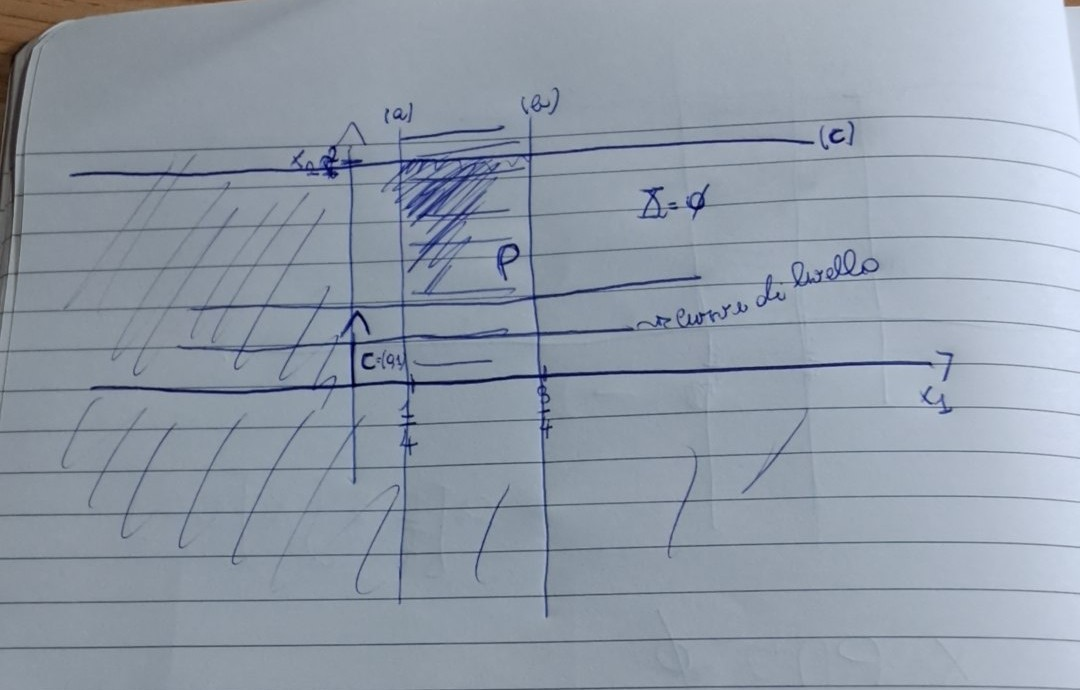
\includegraphics[width=0.8\textwidth]{_files/_images/photo_2026-11-12_17-15-25.jpg}
    \caption{Regione ammissibile del rilassamento nell'esempio:
\(x^*\notin\mathbb Z^2\) e il vettore arrotondato \(x^I\notin X\).
Il problema intero ha \(X=\varnothing\); la freccia della funzione
obiettivo indica il verso di crescita di \(x_2\).}
    \label{fig:immagine}
\end{figure}


\subsection{Relazioni fra un problema di PLI ed il suo rilassamento continuo}

Siano (Pli) un problema di programmazione lineare intera con regione ammissibile $X$, $X^*$ insieme di soluzioni ottime e sia $z^*_{(Pli)}$ il valore ottimo della funzione obiettivo,sempre nel problema di programmazione lineare intera.
Consideriamo poi (Pli-c) il suo rilassamento continuo con regione ammissibile $P$,$P^*$ l'insieme di soluzioni ottime e il valore ottimo della funzione obiettivo del Pli-c, come $z^*_{(Pli-c)}$

\begin{proposition}{Relazioni fondamentali}
Fra il problema intero e il suo rilassamento valgono le seguenti relazioni.
\begin{enumerate}
\item \(P=\varnothing\Longrightarrow X=\varnothing\):
se il rilassamento è inammissibile, lo è anche il problema intero.

\item Se il problema intero è illimitato nel verso di ottimizzazione,
anche il rilassamento è illimitato nello stesso verso.
Per un problema di minimo,
\[
z^*_{(Pli)} = -\infty \implies z^*_{(Pli-c)} = -\infty  
\]
Per un problema di massimo, l'analoga relazione usa \(+\infty\).

\item Se \(P^*\neq\varnothing\) (cioè appartiene all'insieme delle soluzioni ottime) e \(X^*\neq\varnothing\), nel caso
di minimo si ha il lower bound
\[
z^*_{(\mathrm{Pli\text{-}c})}\leq z^*_{(\mathrm{Pli})}.
\]
Questo perchè $P$ è piu grande ed è un sottoinsieme di $X$


\item Se \(y\in P^*\) e \(y\in\mathbb Z^n\), allora
\[
y\in X^*,\qquad
z(y)=z^*_{(\mathrm{Pli\text{-}c})}=z^*_{(\mathrm{Pli})}.
\]

\item Può accadere che
\[
X=\varnothing,\qquad P^*\neq\varnothing.
\]
È il caso dell'esempio precedente: il problema intero è inammissibile,
ma il rilassamento possiede un ottimo finito.

\item Può accadere che \(X=\varnothing\) e il rilassamento sia illimitato.
Un esempio è
\begin{align*}
\max\quad &x_2\\
\text{s.a.}\quad
&x_1\geq\frac14 &&\text{(a)},\\
&x_1\leq\frac34 &&\text{(b)},\\
&x_1,x_2\geq0,\qquad x_1,x_2\in\mathbb Z.
\end{align*}
Qui \(X=\varnothing\), mentre nel rilassamento continuo il valore della funzione obiettivo può crescere illimitatamente verso + $\infty$.
Questo perchè la regione ammissibile $P$ è illimtata verso l'alto, come vedi sotto.
\end{enumerate}
\end{proposition}



\begin{center}
\begin{minipage}{\linewidth}
\centering
\captionsetup{hypcap=false}
\begin{tikzpicture}[x=3.8cm,y=1.2cm,>=Stealth,font=\small]
  \fill[blue!7] (.25,0) rectangle (.75,3.2);
  \draw[->] (-.13,0)--(1.65,0) node[right] {$x_1$};
  \draw[->] (0,-.25)--(0,3.3) node[above] {$x_2$};
  \draw[->] (.25,-.12)--(.25,3.15) node[above] {(a)};
  \draw[->] (.75,-.12)--(.75,3.15) node[above] {(b)};
  \draw[->] (.25,2.8)--(.43,2.8);
  \draw[->] (.75,2.6)--(.57,2.6);
  \draw[brown!70!black] (-.1,1.6)--(1.5,1.6);
  \draw[->,brown!70!black] (1.4,1.6)--(1.4,2)
    node[right] {f.o.};
  \foreach \x/\lab in {.25/{\frac14},.5/{\frac12},.75/{\frac34},1/1} {
    \draw (\x,.035)--(\x,-.035);
    \node[below] at (\x,-.04) {$\lab$};
  }
  \foreach \y in {1,2} \node[left] at (0,\y) {$\y$};
  \node at (.5,1.1) {$P$};
  \node at (1.12,.65) {$X=\varnothing$};
\end{tikzpicture}
\captionof{figure}{Regione del rilassamento nel caso 6: la striscia
\(\frac14\leq x_1\leq\frac34,\ x_2\geq0\) è illimitata verso l'alto
ma non contiene punti interi. Quindi \(X=\varnothing\), mentre
il rilassamento di massimo ha valore \(+\infty\).}
\label{fig:striscia-illimitata}
\end{minipage}
\end{center}

\subsection{Matrice dei vincoli unimodulare}
\label{subsec:unimodularita}

In generale l'ottimo del rilassamento non risolve direttamente
il problema intero. Esistono però strutture della matrice dei vincoli
che garantiscono l'interezza delle soluzioni di base, quando
i termini noti sono interi.

\begin{definition}{Matrice unimodulare}
Una matrice intera \(A\in\mathbb Z^{m\times n}\), con \(m\leq n\),
si dice \emph{unimodulare}, nella terminologia adottata nel testo,
se ogni sua sottomatrice quadrata \(B\in\mathbb Z^{m\times m}\)
soddisfa
\[
\det(B)\in\{-1,0,1\}.
\]
\end{definition}


Supponiamo di dover risolvere un problema di programmazione lineare intera (Pli), in cui la matrice dei vincoli \(A\) e il vettore dei termini noti \(b\) abbiano elementi interi.

Consideriamo ora il rilassamento continuo associato al problema (Pli) e supponiamo che \(x^*\) sia una sua soluzione ottima del problema.

Vogliamo stabilire sotto quali condizioni \(x^*\) abbia tutte le componenti intere, così da poter concludere che \(x^*\) è anche una soluzione ottima del problema originale (Pli).

\begin{warning}{}
  Prima di procedere, ricordati un teorema fondamentale,se un problema di programmazione lineare in forma standard (in questo caso il rilassamento continuo),
  ammette una soluzione ottima, allora esiste almeno una soluzione ottima che è una soluzione di base ammissibile (SBA).
\end{warning}

Noi quindi stiamo considerando $x^*$ come una soluzione ottima del problema, questa può essere o una soluzione ottima, o una SBA se è un vertice del poliedro, ma non una SB, perchè se fosse una SB e anche ottima, questo richiederebbe l'ammissibilità cioè sarebbe una SBA ottima.


Consideriamo quindi $x^*$,una SBA (dato che sappiamo che esiste dal teorema) (una SBA cioè stiamo considerando un vertice del poliedro), dato che una SBA è una soluzione di base, allora possiamo applicare il teorema \ref{teorema SBA}

\begin{warning}{}
  Nota che questo procedimento (cioè per dimostrare l'integrità) si può applicare a qualsiasi SBA, non perforza a SBA ottime del problema.
\end{warning}

Se \(B\) è la matrice di base associata alla soluzione $x^*$,
\[
x^*=
\begin{bmatrix}x_B^*\\x_N^*\end{bmatrix}
=
\begin{bmatrix}B^{-1}b\\0\end{bmatrix}.
\]
Le componenti non di base sono già intere perché nulle.
L'interezza di \(x^*\) dipende dunque da \(B^{-1}b\).
Poiché \(b\in\mathbb Z^m\) (abbiamo presupposto che $A$ e $b$ fossero interi), una condizione sufficiente è che
\(B^{-1}\) sia intera.

Per definizione si ha che:
\[
B^{-1}
=\frac{1}{\det(B)}
\begin{bmatrix}
\alpha_{11}&\alpha_{12}&\cdots&\alpha_{1m}\\
\alpha_{21}&\alpha_{22}&\cdots&\alpha_{2m}\\
\vdots&\vdots&\ddots&\vdots\\
\alpha_{m1}&\alpha_{m2}&\cdots&\alpha_{mm}
\end{bmatrix}^{\mathsf T},
\]
dove
\[
\alpha_{ij}=(-1)^{i+j}\det(M_{ij})
\]
e \(M_{ij}\) si ottiene da \(B\) eliminando la riga \(i\)
e la colonna \(j\).

La matrice \(B\) è intera perché è estratta da \(A\).
Ogni \(M_{ij}\) è intera, quindi il suo determinante (det($M_{i,j}$)) e
il cofattore \(\alpha_{ij}\) sono interi.

Quindi $B^{-1}$ è intera se il determinante di $B$ è -1 o 1:
\[
\det(B)\in\{-1,1\},
\]

Quindi :
\[
\det(B)\in\{-1,1\} \implies x^* \in \mathbb{Z}^n
\]
E quindi $x^*$ è una soluzione ottima anche del problema originale.
\textbf{$x^*$ era una SBA e quindi un vertice del poliedro del problema di rilassamento, e abbiamo dimostrato che era intero}

Da questo possiamo generalizzare a tutti i vertici del poliedro e dire questo teorema:
\begin{theorem}{Interezza dei vertici}
\label{thm:vertici-interi}
Sia \(A\in\mathbb Z^{m\times n}\) unimodulare e di rango \(m\),
e sia \(b\in\mathbb Z^m\). Allora il poliedro
\[
P=\{x\in\mathbb R^n:Ax=b,\ x\geq0\}
\]
ha soltanto vertici interi.
\end{theorem}

\begin{proof}
Ogni vertice del poliedro in forma standard è una soluzione
di base ammissibile. La sua matrice di base \(B\) è non singolare (cioè il determinante è diverso da 0, questo per la definizione di prima della matrice inversa, dato che il determinante sta del denominatore)
e, dato che per l'unimodularità di \(A\) allora il determinante può assumere questi valori,
\[
\det(B)\in\{-1,0,1\}\setminus\{0\}=\{-1,1\}.
\]
Grazie a prima possiamo dire che  \(B^{-1}\) è intera.
Segue \(x_B=B^{-1}b\in\mathbb Z^m\); inoltre \(x_N=0\).
Ogni vertice appartiene quindi a \(\mathbb Z^n\).
\end{proof}


Se il rilassamento ha un ottimo finito, se ne può scegliere uno
di base: sotto le ipotesi del teorema è intero e risolve
anche il problema di PLI.


\newpage

\subsubsection*{Esempi di problemi di PLI con matrice dei vincoli unimodulare}

Due problemi classici hanno una struttura particolarmente favorevole:
il \emph{Problema del Trasporto} e il \emph{Problema dell'Assegnamento}.
In entrambi i termini noti sono interi e la matrice dei vincoli
possiede una proprietà ancora più forte dell'unimodularità,
che sarà dimostrata di seguito.

\subsubsection{Il Problema del Trasporto: problema di Hitchcock}
\label{ex:trasporto}
Sono dati \(m\) fornitori di un bene \(M\) e \(n\) clienti.
Il fornitore \(i\), con \(i=1,\ldots,m\), dispone di
\(s_i\in\mathbb Z_{\geq0}\) unità di bene; il cliente \(j\),
con \(j=1,\ldots,n\), richiede \(d_j\in\mathbb Z_{\geq0}\) unità.
Il costo di trasporto di un'unità dal fornitore \(i\) al cliente \(j\)
è \(c_{ij}\). Si assume inizialmente il \emph{bilanciamento}:
\begin{equation}
\sum_{i=1}^m s_i=\sum_{j=1}^n d_j.
\tag{3.1}\label{eq:bilanciamento}
\end{equation}
\textbf{cioè c'è merce per tutti, ma senza ecceddere}.\\

L'obiettivo è minimizzare il \textbf{costo totale del trasporto rispettando}
le disponibilità dei fornitori e le richieste dei clienti.

Indichiamo con \(f_{ij}\) la quantità \textbf{trasportata} dal fornitore \(i\) al cliente \(j\).
La formulazione è
\begin{align*}
\min\quad &\sum_{i=1}^m\sum_{j=1}^n c_{ij}f_{ij} = c_{11} f_{11} + c_{12} f_{12} \dots \text{ $c$ è un pò come un termine di peso, fissato all'inizio}\\
\text{s.a.}\quad
&\sum_{i=1}^m f_{ij}=d_j \text{ cioè i clienti vengono soddisfati tutti},
&&j=1,\ldots,n \quad \text{(a)},\\
&\sum_{j=1}^n f_{ij}=s_i \text{ cioè i fornitori devono usare tutto il loro bene disponibile e darlo ai clienti},
&&i=1,\ldots,m \quad \text{(b)},\\
&f_{ij}\geq0,
i=1,\ldots,m,j=1,\ldots,n.
\end{align*}


\begin{warning}{}
    Ovviamente, possono esistere diverse soluzioni ammissibili al problema, che differiscono per le quantità di merce trasportate lungo i vari percorsi. Dobbiamo quindi determinare quanta merce trasportare da ciascun fornitore a ciascun cliente, rispettando i vincoli di disponibilità e di domanda, in modo da minimizzare il costo totale del trasporto.
\end{warning}
\begin{observation}{}
    Ogni valore assunto dall'indice $j=1,\dots,n$ identifica un vincolo distinto e, di conseguenza, una riga della matrice $A$.

    In particolare, a $j=1$ corrisponde il primo vincolo, a $j=2$ il secondo, e così via, fino a ottenere $n$ vincoli.

    Analogamente, ogni valore dell'indice $i=1,\dots,m$ identifica un ulteriore vincolo, per un totale di $m$ vincoli.

    Complessivamente, si ottengono quindi $m+n$ vincoli, corrispondenti alle $m+n$ righe della matrice $A$.
\end{observation}

I vincoli (a) sono i \emph{vincoli di destinazione}, cioè che il cliente riceve tutto quello che richiede da i diversi fornitori (può essere anche uno solo) ad es.
\[
d_1 = f_{11} + f_{21} + \dots
\]
Cioè la richiesta di quel cliente, può essere fornita da diversi fornitori


i vincoli (b) sono i \emph{vincoli di origine} cioè che i fornitori forniscano tutto quello che hanno ai clienti (posso fornire anche tutto ad un solo cliente) ad es. 
\[
s_1 = f_{11} + f_{12} + \dots
\]
cioè il fornitore da tutto quello che ha ai vari clienti.




Quello che vogliamo determinare attraverso la risoluzione del problema è il vettore delle variabili decisionali $f$, che in questo caso svolge il ruolo del vettore $x$ di un generico problema di programmazione lineare.

In particolare, vogliamo trovare un vettore $f$ che specifichi quanta merce trasportare lungo ciascun percorso fornitore-cliente, in modo da minimizzare il costo totale del trasporto, rispettando tutti i vincoli del problema.

Il vettore $f$ ha dimensione $mn$, poiché contiene una variabile $f_{ij}$ per ogni possibile coppia fornitore-cliente, con $i=1,\dots,m$ e $j=1,\dots,n$.



\newpage

Si osservi quanto segue.
\begin{enumerate}
\item[i.] Le variabili di decisione $f_{ij}$ sono $m \times n$.
\begin{observation}{}
  Questo perchè per ogni fornitore, dobbiamo modellare con le variabili di decisione $n$ clienti, ad esempio per il fornitore 1, abbiamo:
  \[
  f_{11},f_{12},\dots,f_{1n}
  \]
  ci sono $m$ fornitori e quindi abbiamo $m \times n$ variabili.
\end{observation}

\item[ii.] Sommando i vincoli di destinazione e quelli di origine,
\[
\sum_{j = 1}^{n} \sum_{i = 1}^{m} f_{ij} = \sum_{i = 1}^{m} \sum_{j = 1}^{n} f_{ij} \implies \sum_{j = 1}^{n} d_j = \sum_{i = 1}^{m} s_i  
\]
Il bilanciamento \eqref{eq:bilanciamento} è quindi necessario
per l'ammissibilità del modello con tutte le uguaglianze.

\item[iii.] La matrice dei vincoli è unimodulare e
con \(s_i,d_j\) interi, ogni soluzione di base ammissibile
è intera (\textbf{dal teorema di interezza dei vertici}).


\begin{definition}{Grafo Bipartito}
Un grafo bipartito è un grafo \(G=(V,E)\) in cui l'insieme dei vertici \(V\) può essere suddiviso in due sottoinsiemi disgiunti \(V_1\) e \(V_2\), tali che:
\begin{enumerate}
  \item \(V_1 \cup V_2 = V\)
  \item \(V_1 \cap V_2 = \varnothing\)
  \item Ogni arco collega un vertice di \(V_1\) con un vertice di \(V_2\).
\end{enumerate}
Un grafo è Bipartito completo, se ogni vertice di \(V_1\) è collegato a ogni vertice di \(V_2\)
\end{definition}

\item[iv.] Ogni istanza si rappresenta con un grafo bipartito completo, l'istanza del grafo è:
\[
K_{m,n}=(F\cup C,E),
\]
nel quale:
\begin{itemize}
\item \(F=\{1,\ldots,m\}\) è l'insieme dei fornitori;
\item \(C=\{1,\ldots,n\}\) è l'insieme dei clienti, distinto da \(F\);
\item \(E=\{[i,j]:i\in F,\ j\in C\}\);
\item \(c:E\longrightarrow\mathbb R_{\geq0}\) associa
il costo \(c_{ij}\) al collegamento \([i,j]\).
\end{itemize}
Le frecce nelle figure indicano il trasporto dal fornitore
al cliente.
\end{enumerate}

\begin{center}
\begin{minipage}{\linewidth}
\centering
\captionsetup{hypcap=false}
\begin{tikzpicture}[>=Stealth,font=\small,
  forn/.style={circle,draw=blue!65!black,minimum size=7mm,inner sep=1pt},
  cli/.style={circle,draw=red!70!black,minimum size=7mm,inner sep=1pt}]
  \node[forn] (f1) at (0,3.6) {$1$};
  \node[forn] (fi) at (0,1.8) {$i$};
  \node[forn] (fm) at (0,0) {$m$};
  \node[cli] (c1) at (5,3.6) {$1$};
  \node[cli] (cj) at (5,1.8) {$j$};
  \node[cli] (cn) at (5,0) {$n$};
  \node[above,blue!65!black] at (f1.north) {$F$};
  \node[above,red!70!black] at (c1.north) {$C$};
  \foreach \f in {f1,fi,fm}
    \foreach \c in {c1,cj,cn}
      \draw[->,gray!75] (\f)--(\c);
  \draw[->] (fi)--node[above,fill=white,inner sep=2pt] {$c_{ij}$}(cj);
  \node at (0,2.7) {$\vdots$};
  \node at (0,.9) {$\vdots$};
  \node at (5,2.7) {$\vdots$};
  \node at (5,.9) {$\vdots$};
\end{tikzpicture}
\captionof{figure}{Grafo bipartito completo rappresentante una generica istanza
del Problema del Trasporto. Ogni fornitore è collegato a ogni cliente;
il collegamento \([i,j]\) ha costo \(c_{ij}\).}
\label{fig:trasporto-generico}
\end{minipage}
\end{center}

La matrice dei coefficienti tecnologici ha dimensioni
\[
(m+n)\times mn
\]
\begin{warning}{}
    Questo perché:
    \begin{enumerate}
        \item \textbf{Numero di righe: $m+n$.}
        Ogni riga della matrice corrisponde a un vincolo del problema.
        In particolare:
        \begin{itemize}
            \item Abbiamo $n$ vincoli relativi alla domanda dei clienti, uno per ciascun cliente $j=1,\dots,n$.
            \item Abbiamo $m$ vincoli relativi alla disponibilità dei fornitori, uno per ciascun fornitore $i=1,\dots,m$.
        \end{itemize}
        Pertanto, il numero complessivo di righe è $m+n$.

        \item \textbf{Numero di colonne: $mn$.}
        Ogni colonna corrisponde a una variabile decisionale $f_{ij}$, che rappresenta la quantità di merce trasportata dal fornitore $i$ al cliente $j$.

        Poiché abbiamo $m$ fornitori e $n$ clienti, esistono $mn$ possibili coppie fornitore-cliente e, quindi, $mn$ variabili decisionali.

        Questo rappresenta tutte le possibili coppie fornitore-clienti che possono essere messe sulle colonne
    \end{enumerate}
\end{warning}
e coincide con la matrice di incidenza nodo--arco \emph{non orientata}
del grafo bipartito

Consideriamo concretamente \(m=3\) fornitori e \(n=2\) clienti:
\begin{align*}
\min\quad
&c_{11}f_{11}+c_{12}f_{12}
+c_{21}f_{21}+c_{22}f_{22}
+c_{31}f_{31}+c_{32}f_{32}\\
\text{s.a.}\quad
&f_{11}+f_{12}=s_1,\\
&f_{21}+f_{22}=s_2,\\
&f_{31}+f_{32}=s_3,\\
&f_{11}+f_{21}+f_{31}=d_1,\\
&f_{12}+f_{22}+f_{32}=d_2,\\
&f_{ij}\geq0,\qquad i=1,2,3,\quad j=1,2.
\end{align*}
Nell'ordine di colonne
\[
f_{11},\ f_{12},\ f_{21},\ f_{22},\ f_{31},\ f_{32},
\]
la matrice è
\[
A=
\begin{bmatrix}
1&1&0&0&0&0\\
0&0&1&1&0&0\\
0&0&0&0&1&1\\
1&0&1&0&1&0\\
0&1&0&1&0&1
\end{bmatrix}\in\mathbb Z^{5\times6}.
\]
il vettore decisionale è
\[
f = \begin{pmatrix}
f_{11} \\
 f_{12} \\
 \vdots \\
 f_{mn}
\end{pmatrix}
\]

Le prime tre righe rappresentano i fornitori, le ultime due
i clienti. Il grafo associato è \(K_{3,2}\), con
\(F=\{1,2,3\}\) e \(C=\{1,2\}\).

\begin{center}
\begin{minipage}{\linewidth}
\centering
\captionsetup{hypcap=false}
\begin{tikzpicture}[>=Stealth,font=\small,
  forn/.style={circle,draw=blue!65!black,minimum size=8mm},
  cli/.style={circle,draw=red!70!black,minimum size=8mm}]
  \node[forn] (f1) at (0,4) {$1$};
  \node[forn] (f2) at (0,2) {$2$};
  \node[forn] (f3) at (0,0) {$3$};
  \node[cli] (c1) at (5,3.5) {$1$};
  \node[cli] (c2) at (5,.5) {$2$};
  \node[above,blue!65!black] at (f1.north) {$F$};
  \node[above,red!70!black] at (c1.north) {$C$};
  \draw[->] (f1)--node[pos=.35,above,fill=white,inner sep=1pt] {$c_{11}$}(c1);
  \draw[->] (f1)--node[pos=.25,below,fill=white,inner sep=1pt] {$c_{12}$}(c2);
  \draw[->] (f2)--node[pos=.3,above,fill=white,inner sep=1pt] {$c_{21}$}(c1);
  \draw[->] (f2)--node[pos=.32,below,fill=white,inner sep=1pt] {$c_{22}$}(c2);
  \draw[->] (f3)--node[pos=.24,above,fill=white,inner sep=1pt] {$c_{31}$}(c1);
  \draw[->] (f3)--node[pos=.35,below,fill=white,inner sep=1pt] {$c_{32}$}(c2);
\end{tikzpicture}
\captionof{figure}{Grafo \(K_{3,2}\) dell'istanza del trasporto con tre fornitori
e due clienti. Sono rappresentati tutti i sei collegamenti
e i rispettivi costi.}
\label{fig:trasporto-32}
\end{minipage}
\end{center}

\newpage

\paragraph{Importanti osservazioni.}

La prima importante osservazione riguarda l'ipotesi di bilanciamento, che risulta essere non restrittiva.

Questo significa che, anche qualora il problema originale non fosse bilanciato, sarebbe comunque possibile ricondurlo a un problema bilanciato equivalente, senza compromettere la ricerca di una soluzione ottima.

Si considerino, infatti, i seguenti due scenari alternativi:


\paragraph{Scenario 1: offerta complessiva inferiore alla domanda}
Supponiamo che
\[
\sum_{i=1}^m s_i<\sum_{j=1}^n d_j.
\]
I fornitori reali non possono soddisfare tutta la domanda.
Per i soli flussi reali si considera quindi
\[
\sum_{i=1}^m f_{ij}\leq d_j,\qquad j=1,\ldots,n.
\]
Cioè per alcuni clienti potrebbe essere minore, per alcuni uguale e soddisfarli.


Questo non va bene perchè non rispetta il vincolo (a) che avevamo messo nel problema standard, quindi faremo in modo di bilanciarlo. 
\\
\textbf{Questo viola il vincolo (a), quindi come si fa a bilanciarlo?}
\\
Si procede così:
\begin{enumerate}
\item si introduce un fornitore fittizio \(m+1\) nell'insieme dei fornitori;
\item si introducono \(n\) ulteriori variabili
\[
f_{(m+1)j}\geq0,\qquad j=1,\ldots,n;
\]
\item si definiscono la disponibilità del nuovo fornitore fittizio e i suoi costi:
\[
\begin{aligned}
s_{m+1} &= \sum_{j=1}^n d_j-\sum_{i=1}^m s_i,
\\
\\[6pt]
c_{(m+1)j} &= \text{da definire},\qquad j=1,\ldots,n.
\end{aligned}
\]
cioè la disponibilità del fornitore fittizio viene definita come la quantità di merce necessaria a soddisfare la domanda complessiva che non può essere coperta dagli altri fornitori.
\end{enumerate}
Il modello bilanciato risultante è
\begin{align*}
\min\quad &\sum_{i=1}^{m+1}\sum_{j=1}^n c_{ij}f_{ij}\\
\text{s.a.}\quad
&\sum_{j=1}^n f_{ij}=s_i,
&&i=1,\ldots,m+1 \qquad\text{(a)},\\
&\sum_{i=1}^{m+1}f_{ij}=d_j,
&&j=1,\ldots,n \qquad\text{(b)},\\
&f_{ij}\geq0,
&&i=1,\ldots,m+1,\quad j=1,\ldots,n.
\end{align*}
La quantità \(f_{(m+1)j}\) che compare sopratutto nel vincolo (a) misura la domanda del cliente \(j\)
non soddisfatta dai fornitori reali. Questo perchè devi pensarlo cosi, quando arriva $i=m+1$, si ha
\[
s_{m+1} = f_{m+1,1} + f_{m+1,2} + \dots + f_{m+1,n}
\]
ed ognuno misura la quantità non soddisfata dai fornitori reali, che verrà soddisfatta da questo.


\newpage

\paragraph{Scenario 2: offerta complessiva superiore alla domanda}
Supponiamo che
\[
\sum_{i=1}^m s_i>\sum_{j=1}^n d_j.
\]
Cioè la disponibilità di fornitura, è maggiore della domanda degli utenti.


Succede quindi che \textbf{qualche} fornitore può spedire meno della propria disponibilità:
\[
\sum_{j=1}^n f_{ij}\leq s_i,\qquad i=1,\ldots,m.
\]
Cioè un fornitore spartenedo la sua merce a tutti i clienti potrebbe non esaurire la quantità che ha disposizione.
\textbf{Questo viola il vincolo (b), quindi come si fa a bilanciarlo?}
\\
Si procede così:
\begin{enumerate}
\item si introduce un cliente fittizio \(n+1\);
\item si introducono \(m\) ulteriori variabili
\[
f_{i(n+1)}\geq0,\qquad i=1,\ldots,m;
\]
\item si definiscono la sua domanda e i suoi costi:
\[
d_{n+1}=\sum_{i=1}^m s_i-\sum_{j=1}^n d_j,
\qquad
c_{i(n+1)}\ \text{da definire},\quad i=1,\ldots,m.
\]
\textbf{Questo cliente quindi prenderà tutto quello che hanno in piu gli altri fornitori}
\end{enumerate}
Il modello bilanciato è
\begin{align*}
\min\quad &\sum_{i=1}^m\sum_{j=1}^{n+1}c_{ij}f_{ij}\\
\text{s.a.}\quad
&\sum_{j=1}^{n+1}f_{ij}=s_i,
&&i=1,\ldots,m \qquad\text{(a)},\\
&\sum_{i=1}^m f_{ij}=d_j,
&&j=1,\ldots,n+1 \qquad\text{(b)},\\
&f_{ij}\geq0,
&&i=1,\ldots,m,\quad j=1,\ldots,n+1.
\end{align*}
Il flusso verso il cliente fittizio rappresenta l'offerta inutilizzata.
Il relativo costo può essere nullo oppure descrivere, per esempio,
costi di stoccaggio o smaltimento.


\textbf{Quindi in tutti e due i casi abbiamo bilanciato il problema, facendo in modo che rispettasero i vincoli (a) e (b)}


La seconda osservazione riguarda l'esistenza di un ottimo finito.

\newpage

\begin{theorem}{Esistenza di un ottimo finito per il trasporto}
\label{thm:trasporto-ottimo}
Ogni istanza \textbf{bilanciata} del Problema del Trasporto
ammette almeno una soluzione ottima finita.
\end{theorem}

\begin{proof}
Poniamo
\[
\alpha=\sum_{i=1}^m s_i=\sum_{j=1}^n d_j.
\]
Definiamo
\begin{equation}
f_{ij}=\frac{s_i d_j}{\alpha},
\qquad i=1,\ldots,m,\quad j=1,\ldots,n.
\tag{3.2}\label{eq:soluzione-proporzionale}
\end{equation}
Tali quantità sono nonnegative. Ora abbiamo dato un assegnamento alla quantità trasportata, vediamo se queste quantità soddisfano i vincoli.
Per ogni fornitore \(i\), i vincoli di origine sono soddisfatti:
\begin{align*}
\sum_{j=1}^n f_{ij}
&=\sum_{j=1}^n\left(\frac{s_i d_j}{\sum_{r=1}^m s_r}\right)\\
&=\frac{s_i}{\sum_{r=1}^m s_r}\sum_{j=1}^n d_j\\
&=\frac{s_i}{\alpha}\,\alpha
\qquad\text{per il bilanciamento}\\
&=s_i.
\end{align*}
Per ogni cliente \(j\), i vincoli di destinazione sono soddisfatti:
\begin{align*}
\sum_{i=1}^m f_{ij}
&=\sum_{i=1}^m\left(\frac{s_i d_j}{\sum_{\ell=1}^n d_\ell}\right)\\
&=\frac{d_j}{\sum_{\ell=1}^n d_\ell}\sum_{i=1}^m s_i\\
&=\frac{d_j}{\alpha}\,\alpha
\qquad\text{per il bilanciamento}\\
&=d_j.
\end{align*}
La soluzione \eqref{eq:soluzione-proporzionale} è ammissibile.
Quindi abbiamo dimostrato che la regione ammissibile è non vuota e può contenere questa soluzione, quindi sicuramente è non vuota.


Poi per ogni soluzione ammissibile (immagina ce ne siano tante) e per ogni \(i,j\), si ha inoltre
\begin{align*}
&f_{ij}\geq0,\\
&\sum_{j=1}^n f_{ij}=s_i
\quad\Longrightarrow\quad f_{ij}\leq s_i, \forall i,j\\
&\sum_{i=1}^m f_{ij}=d_j
\quad\Longrightarrow\quad f_{ij}\leq d_j \forall i,j.
\end{align*}
Quindi
\[
0\leq f_{ij}\leq\min\{s_i,d_j\}.
\]
La funzione obiettivo, essendo lineare, è continua. Poiché la regione ammissibile è non vuota e compatta, per il teorema di Weierstrass la funzione obiettivo assume su di essa un minimo e un massimo assoluti. Di conseguenza, possiamo affermare che esiste almeno una soluzione ottima finita, anche se non sappiamo ancora quale sia
\end{proof}


\newpage
La terza osservazione riguarda la matrice dei coefficienti tecnologici.
Per il trasporto si può dimostrare la \emph{totale unimodularità},
che riguarda tutti i minori quadrati, non soltanto quelli
di ordine massimo.

\begin{definition}{Matrice totalmente unimodulare}
Una matrice intera \(A\in\mathbb Z^{m\times n}\), con \(m\leq n\),
si dice \emph{totalmente unimodulare} se, per \textbf{ogni sottomatrice
quadrata} \(B\) di qualunque ordine \(k=1,\ldots,m\), vale
\[
\det(B)\in\{-1,0,1\}.
\]

\end{definition}

\begin{remark}{Chiarimento sulla differenza fra le due proprietà}
La totale unimodularità implica l'unimodularità nella definizione.
\end{remark}

\begin{theorem}{Totale unimodularità della matrice del trasporto}
\label{thm:trasporto-tu}
Sia \(A\) la matrice dei coefficienti tecnologici del Problema
del Trasporto. Per ogni sua sottomatrice quadrata \(A^{(k)}\)
di ordine \(k\), vale
\[
\det\!\left(A^{(k)}\right)\in\{-1,0,1\}.
\]
Quindi \(A\) è totalmente unimodulare.
\end{theorem}

\begin{proof}
Ogni colonna di \(A\), corrispondente a \(f_{ij}\), contiene
esattamente due \(1\): uno in una riga di origine e uno
in una riga di destinazione. Gli altri elementi sono nulli.
Una colonna di \(A^{(k)}\) può dunque contenere zero, uno o due \(1\).

Procediamo per induzione sull'ordine \(k\). Per \(k=1\), l'elemento
è \(0\) o \(1\), quindi l'affermazione è vera.
Per \(k>1\), distinguiamo i tre casi del testo.
\begin{enumerate}
\item \textbf{Esiste una colonna interamente nulla.}, basta che una fra le colonne è interamente nulla
Il determinante è immediatamente nullo:
\[
\det\!\left(A^{(k)}\right)=0.
\]

\item \textbf{Ogni colonna contiene due \(1\).}
Sono presenti entrambi gli estremi di ciascun arco selezionato.
La somma delle righe di origine coincide con quella
delle righe di destinazione: ciascuna colonna contribuisce
con un \(1\) a entrambe. Le righe sono linearmente dipendenti
e il determinante è nullo.

L'esempio del testo, con tre fornitori e due clienti, è
\[
A=
\begin{bmatrix}
1&1&0&0&0&0\\
0&0&1&1&0&0\\
0&0&0&0&1&1\\
1&0&1&0&1&0\\
0&1&0&1&0&1
\end{bmatrix}
\quad\Longrightarrow\quad
A^{(4)}=
\begin{bmatrix}
1&1&0&0\\
0&0&1&1\\
1&0&1&0\\
0&1&0&1
\end{bmatrix}.
\]
Le prime due righe di \(A^{(4)}\) sono di origine e le ultime
due di destinazione. Le somme sono
\[
\begin{array}{rrrr@{\quad}c}
1&1&0&0&+\\
0&0&1&1&\\ \cline{1-4}
1&1&1&1&
\end{array}
\qquad\qquad
\begin{array}{rrrr@{\quad}c}
1&0&1&0&+\\
0&1&0&1&\\ \cline{1-4}
1&1&1&1&
\end{array}.
\]
Ne segue
\[
\text{riga}_1+\text{riga}_2-\text{riga}_3-\text{riga}_4=0,
\qquad \det\!\left(A^{(4)}\right)=0.
\]
Lo stesso ragionamento vale per qualunque \(k\) in questo caso.

\item \textbf{$A^{(k)}$ non ha alcuna colonna di tutti "0", ma almeno una colonna (eventualmente tutte) con un solo "1" (quindi eventualmente altre colonne possono avere tutti "1").}
Sviluppiamo il determinante lungo una di tali colonne.
Se l'\(1\) scelto (bisogna scegliere perforza un 1,per la regola del determinante) è nella posizione \((r,s)\), lo sviluppo
di Laplace dà
\[
\det\!\left(A^{(k)}\right)
=(-1)^{r+s}\det\!\left(A^{(k-1)}\right).
\]
Per solo ipotesi induttiva, \(\det\!\left(A^{(k-1)}\right)\in\{-1,0,1\}\); quindi anche
\(\det\!\left(A^{(k)}\right)\in\{-1,0,1\}\).

\end{enumerate}

\begin{example}{Esempio del terzo caso}
    
    \textbf{Esiste una colonna contenente esattamente
    un elemento uguale a $1$.}

    Escludendo i due casi precedenti, deve necessariamente
    esistere almeno una colonna contenente un solo $1$.

    In questo caso possiamo applicare lo
    \textbf{sviluppo di Laplace} lungo tale colonna,
    riducendo il calcolo del determinante a quello
    di una sottomatrice di ordine $k-1$.

    Consideriamo, ad esempio:

    \[
    A^{(3)}=
    \begin{pmatrix}
    0 & 1 & 1\\
    1 & 0 & 1\\
    0 & 1 & 0
    \end{pmatrix}.
    \]

    Osserviamo che la prima colonna contiene
    un solo elemento uguale a $1$, situato
    nella seconda riga.

    Sviluppando il determinante lungo questa colonna:

    \[
    \begin{aligned}
    \det(A^{(3)})
    &=(-1)^{2+1}
    \det
    \begin{pmatrix}
    1 & 1\\
    1 & 0
    \end{pmatrix}\\[6pt]
    &=-\left(1\cdot 0-1\cdot 1\right)\\[6pt]
    &=-(-1)\\[6pt]
    &=1.
    \end{aligned}
    \]

    Abbiamo quindi ottenuto:

    \[
    \boxed{\det(A^{(3)})=1.}
    \]

\textbf{Conclusione.}

I tre casi esaminati coprono tutte le possibilità,
poiché ogni colonna di $A^{(k)}$ può contenere
al massimo due elementi uguali a $1$.

Il caso base $k=1$ è immediato, poiché ogni
elemento della matrice originale appartiene
a $\{0,1\}$.

Per induzione, ogni sottomatrice quadrata
di $A$ ha determinante appartenente a
$\{-1,0,1\}$.

Possiamo quindi concludere che:

\[
\boxed{A \text{ è totalmente unimodulare}.}
\]

\end{example}

Quindi abbiamo dimostrato che ogni matrice quadrata che prendiamo (con $k > 1$), può ricadere nei 3 casi.

Nei primi due casi, è semplici da gestire, nell'ultimo caso si usa l'ipotesi di induzione.
\end{proof}

\begin{corollary}{Interezza delle soluzioni di base del trasporto}
\label{cor:trasporto-intero}
Se per ogni $i = 1,\dots,m$ e per ogni $j = 1,\dots,n$ si ha che $s_i$ e $d_j$ sono interi, allora ogni soluzione di base ammissibile del problema del trasporto è intera. 
\end{corollary}

\paragraph{Il Problema dell'Assegnamento}
\label{ex:assegnamento}
Il Problema dell'Assegnamento è il caso speciale del trasporto in cui:
\begin{enumerate}
\item[i.] \(m=n\): il numero di fornitori coincide con quello dei clienti;
\item[ii.] \(s_i=d_j=1\) per ogni \(i,j=1,\ldots,n\).
\end{enumerate}
La formulazione è
\begin{align*}
\min\quad &\sum_{i=1}^n\sum_{j=1}^n c_{ij}f_{ij}\\
\text{s.a.}\quad
&\sum_{i=1}^n f_{ij}=1,
&&j=1,\ldots,n \qquad\text{(a)},\\
&\sum_{j=1}^n f_{ij}=1,
&&i=1,\ldots,n \qquad\text{(b)},\\
&f_{ij}\geq0,
&&i=1,\ldots,n,\quad j=1,\ldots,n.
\end{align*}
La matrice è totalmente unimodulare e i termini noti
sono interi. Ogni soluzione di base ammissibile è dunque intera.
Dalle somme di riga (dei vincoli (a) e (b)) e dalla nonnegatività segue anche
\[
0\leq f_{ij}\leq1.
\]
Ogni soluzione di\textbf{ base ammissibile} (perchè intera) è perciò un vettore booleano,
con il significato
\[
f_{ij}=
\begin{cases}
1,&\text{se il fornitore \(i\) è assegnato al cliente \(j\)},\\
0,&\text{altrimenti}.
\end{cases}
\]
In particolare in una SBA \emph{intera}, fra le \(n^2\) ($mn$)
variabili esattamente \(n\) valgono \(1\) (\textbf{questo perchè fra gli $n$ clienti, posso ricevere in totale massimo $n$ oggetti}); le altre \(n^2-n\) valgono \(0\).
La matrice \((f_{ij})\) è una matrice di permutazione.

Ogni istanza si rappresenta con
\[
K_{n,n}=(F\cup C,E),
\]
nel quale:
\begin{itemize}
\item \(F=\{1,\ldots,n\}\) rappresenta i fornitori;
\item \(C=\{1,\ldots,n\}\) rappresenta i clienti ed è distinto da \(F\);
\item \(E=\{[i,j]:i\in F,\ j\in C\}\);
\item \(c:E\longrightarrow\mathbb R_{\geq0}\), con \(c([i,j])=c_{ij}\).
\end{itemize}
La matrice dei vincoli coincide con la matrice di incidenza
nodo--arco non orientata del grafo bipartito completo.
Una soluzione intera seleziona \(n\) collegamenti
che coprono ogni nodo una sola volta.

\begin{center}
\begin{minipage}{\linewidth}
\centering
\captionsetup{hypcap=false}
\begin{tikzpicture}[>=Stealth,font=\small,
  forn/.style={circle,draw=blue!65!black,minimum size=7mm},
  cli/.style={circle,draw=red!70!black,minimum size=7mm}]
  \node[forn] (f1) at (0,3.6) {$1$};
  \node[forn] (fi) at (0,1.8) {$i$};
  \node[forn] (fn) at (0,0) {$n$};
  \node[cli] (c1) at (5,3.6) {$1$};
  \node[cli] (cj) at (5,1.8) {$j$};
  \node[cli] (cn) at (5,0) {$n$};
  \node[above,blue!65!black] at (f1.north) {$F$};
  \node[above,red!70!black] at (c1.north) {$C$};
  \foreach \f in {f1,fi,fn}
    \foreach \c in {c1,cj,cn}
      \draw[->,gray!75] (\f)--(\c);
  \draw[->] (fi)--node[above,fill=white,inner sep=2pt] {$c_{ij}$}(cj);
  \node at (0,2.7) {$\vdots$};
  \node at (0,.9) {$\vdots$};
  \node at (5,2.7) {$\vdots$};
  \node at (5,.9) {$\vdots$};
\end{tikzpicture}
\captionof{figure}{Grafo bipartito completo di una generica istanza
del Problema dell'Assegnamento: entrambe le parti hanno \(n\) nodi
e il collegamento \([i,j]\) ha costo \(c_{ij}\).}
\label{fig:assegnamento}
\end{minipage}
\end{center}


\newpage

\section{Metodi dei Piani di Taglio}
\label{sec:piani-taglio}
Si consideri il problema di Programmazione Lineare Intera (Pli). Sia $P$ il poliedro regione ammissibile del suo rilassamento continuo (Pli-c)
e sia $X = P \cap \mathcal{Z}^n$ la regione ammissibile di (Pli). \\
Gli algoritmi appartenenti alla famiglia dei metodi dei piani di taglio iterativamente individuano la soluzione ottima $x^*$ del rilassamento continuo (Pli-c) e se $x^*$ \textbf{ha almeno una componente frazionaria} (quindi non è intero), essi \textbf{individuano un vincolo}
soddisfato da tutte le soluzioni intere del problema appartenenti alla regione ammissibile $P$ (cioè praticamente tutta la regione $X$), ma non soddisfato (\textbf{quindi violato}) dalla soluzione ottima $x^*$.
\textbf{Tale vincolo che abbiamo trovato}, viene aggiunto alla formulazione matematica di (Pli-c) è detto \textbf{taglio}.


In generale viene data la seguente definizione:
\begin{definition}{Taglio}
\label{def:taglio}
Dato \(x^*\in P\), il vincolo
\[
a^{\mathsf T}x\leq b_0
\]
è un taglio per \(x^*\) rispetto a \(X\) se:
\begin{enumerate}
\item[i.] Tutti i punti appartenenti all'insieme \(X\) rispettano il vincolo considerato.,
\[
a^{\mathsf T}x\leq b_0\qquad\forall x\in X;
\]
\item[ii.] è violata dal punto da eliminare,
\[
a^{\mathsf T}x^*>b_0.
\]
\end{enumerate}
\end{definition}

\begin{observation}{}
  Il vincolo, potrebbe essere anche un'uguaglianza o un >=, la prof. usa quello per rispettare una canonicità.
  Ricordarti ovviamente che anche se il (Pli-c) è fatto di altri tipo di vincoli (tipo >=), io posso sempre inserire il mio taglio, basta che rispetti la definizione.
\end{observation}


La prima condizione preserva tutte le soluzioni ammissibili
del problema intero, comprese quelle ottime.
La seconda elimina l'ottimo frazionario corrente.
Individuare un adeguato taglio è il \emph{problema della separazione}
di \(x^*\) da \(X\), che in generale può essere difficile
dal punto di vista computazionale.

\begin{center}
\begin{minipage}{\linewidth}
\centering
\captionsetup{hypcap=false}
\begin{tikzpicture}[x=1.04cm,y=.84cm,>=Stealth,font=\small]
  \fill[blue!5] (0,0)--(4.5,0)--(4.5,4)--(2.25,4.75)--(0,2.5)--cycle;
  \fill[red!14] (2,4.5)--(2.25,4.75)--(3,4.5)--cycle;
  \draw[->] (-.6,0)--(8,0) node[right] {$x_1$};
  \draw[->] (0,-.6)--(0,7.2) node[above] {$x_2$};
  \draw[gray] (-.55,1.95)--(5.1,7.6);
  \draw[gray] (-.55,5.6833)--(8,2.8333);
  \draw[gray] (4.5,-.45)--(4.5,7.2);
  \draw[->,gray] (4.8,7.3)--(5.4,6.7);
  \draw[->,gray] (7.2,3.1)--(7,2.45);
  \draw[->,gray] (-.3,2.2)--(.3,1.6);
  \foreach \i in {0,...,7} {
    \foreach \j in {0,...,6} {
      \fill[gray!55] (\i,\j) circle (1.25pt);
      \ifnum\i<5
        \pgfmathtruncatemacro{\amm}{(\j<=\i+2.5)&&(\j<=5.5-\i/3)}
        \ifnum\amm=1 \fill (\i,\j) circle (1.7pt); \fi
      \fi
    }
  }
  \draw[red!65!black] (-.5,4.5)--(8,4.5)
    node[right] {$a^{\mathsf T}x=b_0$};
  \fill (2.25,4.75) circle (2pt);
  \node[above left] at (2.25,4.75) {$x^*$};
  \foreach \i in {1,...,7} \node[below] at (\i,0) {\i};
  \foreach \j in {1,...,6} \node[left] at (0,\j) {\j};
  \node at (2.65,2.5) {$X$};
\end{tikzpicture}
\captionof{figure}{Il taglio \(a^{\mathsf T}x\leq b_0\) preserva tutti
i punti di \(X\) ed elimina \(x^*\). Nello schema il taglio
è orizzontale e la piccola porzione rossa viene esclusa.}
\label{fig:taglio-generico}
\end{minipage}
\end{center}

I metodi dei piani di taglio differiscono soprattutto per
il modo in cui risolvono il problema della separazione,
cioè per la scelta del vincolo aggiunto a ogni iterazione.
Lo schema generale è il seguente.

\begin{center}
\begin{minipage}{\linewidth}
\centering
\captionsetup{hypcap=false}
\fbox{\begin{minipage}{.94\linewidth}
\small
\textbf{algoritmo cutting-plane}\\[3pt]
\begin{tabular}{@{}r@{\quad}p{.86\linewidth}@{}}
1 & Dato \((\mathrm{Pli})\), trovare un ottimo \(x^*\)
del rilassamento \((\mathrm{Pli\text{-}c})\).\\[2pt]
2 & Porre \((\mathrm{Pli\text{-}c})_0:=(\mathrm{Pli\text{-}c})\),
\(x_0^*:=x^*\), \(k:=0\).\\[2pt]
3 & \textbf{while} \(x_k^*\) non è intero \textbf{do}\\
  & \quad individuare un taglio \(a_k^{\mathsf T}x\leq b_k\)
per \(x_k^*\);\\
  & \quad aggiungerlo a \((\mathrm{Pli\text{-}c})_k\),
ottenendo \((\mathrm{Pli\text{-}c})_{k+1}\);\\
  & \quad trovare un ottimo \(x_{k+1}^*\)
di \((\mathrm{Pli\text{-}c})_{k+1}\);\\
  & \quad porre \(k:=k+1\);\\
  & \textbf{endwhile}
\end{tabular}\\[3pt]
\textbf{end cutting-plane}
\end{minipage}}
\captionof{figure}{Schema del generico algoritmo dei piani di taglio,
con gli stessi passi dello pseudocodice del testo.}
\label{fig:algoritmo-cutting-plane}
\end{minipage}
\end{center}

Se si introduce un taglio per iterazione, il numero di iterazioni
del ciclo coincide con il numero di tagli aggiunti.
Intuitivamente, tagli più profondi possono ridurre il numero
di iterazioni; molti tagli ottenuti con le procedure classiche
eliminano però soltanto piccole porzioni del poliedro.
La profondità geometrica non garantisce, da sola,
un determinato numero di iterazioni.

\begin{remark}{Chiarimento sull'invariante e sulle condizioni dello schema}
Se \(P_k\) è la regione del rilassamento all'iterazione \(k\),
per ogni taglio valido si ha
\[
X\subseteq P_{k+1}\subseteq P_k,
\qquad
P_{k+1}\cap\mathbb Z^n=P_k\cap\mathbb Z^n=X.
\]

La seconda affermazione è vera perchè il vincolo nuovo aggiunto, mantiene dentro tutti i punti $X$. 

Per un problema di minimo con ottimi finiti,
\[
z^*_{(\mathrm{Pli\text{-}c})_0}
\leq z^*_{(\mathrm{Pli\text{-}c})_1}
\leq \cdots \leq z^*_{(\mathrm{Pli})}.
\]
Il miglioramento può non essere stretto, ad esempio in presenza
di ottimi multipli.

Lo pseudocodice presuppone che i rilassamenti considerati
abbiano un ottimo finito. Se, aggiungendo soltanto tagli validi,
un rilassamento diventa inammissibile, anche \(X\) è vuoto.
Se il rilassamento iniziale è illimitato, la sola procedura
scritta sopra non basta a classificare il problema intero.
Infine, lo schema astratto non costituisce di per sé
una dimostrazione di terminazione finita per qualunque
regola di generazione dei tagli.
\end{remark}

\newpage

\section{Branch e Bound}
\begingroup
\newcommand{\BBpli}[1]{\mathrm{PLI}_{#1}}
\newcommand{\BBrel}[1]{\mathrm{PLI}_{#1}\text{-c}}
\newcommand{\BBinc}{z_{\mathrm{opt}}}
\newcommand{\BBsol}{x_{\mathrm{opt}}}
\newcommand{\BBfig}[2]{%
  \par\nobreak\smallskip\nobreak
  {\small\textit{Figura #1 delle dispense.} #2\par}}

\subsection{Enumerazione implicita e partizione del problema}

\begin{definition}{Branch \& Bound}
Il Branch \& Bound (B\&B) è un metodo di enumerazione implicita per la
programmazione lineare intera (PLI), alternativo ai metodi dei piani di
taglio. Applica il principio \emph{divide and conquer}. La ramificazione
(\emph{branching}) suddivide il problema in sottoproblemi interi con
insiemi ammissibili più piccoli. La valutazione mediante limiti
(\emph{bounding}) permette di escludere interi sottoalberi quando nessuna
delle loro soluzioni può migliorare la migliore soluzione già trovata.
\end{definition}

\subsubsection{Una partizione in due sottoproblemi}

Sia $X$ l'insieme delle soluzioni intere ammissibili del problema richiamato
nella figura 3.10 delle dispense e sia $P$ la regione del suo rilassamento
continuo. Nella figura 3.11 il rilassamento ha soluzione ottima
\[
 x^*=\left(\frac32,2\right).
\]
La prima coordinata è frazionaria. Ogni soluzione intera deve avere
$x_1\leq 1$ oppure $x_1\geq 2$, poiché non esistono interi strettamente
compresi fra $1$ e $2$. Si costruiscono dunque due problemi distinti.
Nel primo si aggiunge alla formulazione originaria il solo vincolo
$x_1\leq 1$ e nel secondo il solo vincolo $x_1\geq 2$. Si ottengono
\[
 X_1=\{x\in X:x_1\leq 1\},\qquad X_2=\{x\in X:x_1\geq 2\},
\]
\[
 X_1\cup X_2=X,\qquad X_1\cap X_2=\varnothing.
\]
Entrambi i figli escludono $x^*$, mentre ogni soluzione intera del padre
appartiene a uno e un solo figlio. Indicando con $x^*_{x_1\leq 1}$
e $x^*_{x_1\geq 2}$ le rispettive soluzioni ottime, si sceglie quella
con il valore migliore della funzione obiettivo originaria.

\begin{center}
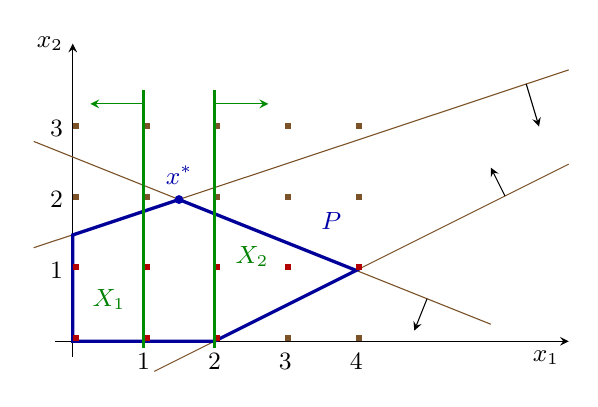
\begin{tikzpicture}[x=.90cm,y=.90cm,>=stealth,font=\small]
  \draw[->] (-.25,0)--(7,0) node[below left] {$x_1$};
  \draw[->] (0,-.22)--(0,4.2) node[left] {$x_2$};
  \draw[brown!65!black] (-.55,1.32)--(7,3.83);
  \draw[brown!65!black] (-.55,2.82)--(5.9,.24);
  \draw[brown!65!black] (1.15,-.425)--(7,2.5);
  \draw[->] (6.4,3.63)--(6.58,3.03);
  \draw[->] (6.1,2.05)--(5.90,2.45);
  \draw[->] (5,.60)--(4.82,.15);
  \draw[blue!60!black,very thick]
    (0,0)--(2,0)--(4,1)--(1.5,2)--(0,1.5)--cycle;
  \foreach \i in {0,...,4}{
    \foreach \j in {0,...,3}{
      \fill[brown!65!black] (\i,\j) rectangle ++(.085,.085);
    }
  }
  \foreach \i/\j in {0/0,0/1,1/0,1/1,2/0,2/1,3/1,4/1}
    \fill[red!70!black] (\i,\j) rectangle ++(.085,.085);
  \foreach \i in {1,2,3,4} \node[below] at (\i,-.04) {$\i$};
  \foreach \j in {1,2,3} \node[left] at (0,\j) {$\j$};
  \foreach \i in {1,2}
    \draw[green!55!black,very thick] (\i,-.10)--(\i,3.55);
  \draw[->,green!55!black] (1,3.35)--(.25,3.35);
  \draw[->,green!55!black] (2,3.35)--(2.76,3.35);
  \fill[blue!65!black] (1.5,2) circle (1.6pt) node[above=2pt] {$x^*$};
  \node[green!50!black] at (.51,.59) {$X_1$};
  \node[green!50!black] at (2.53,1.20) {$X_2$};
  \node[blue!65!black] at (3.65,1.70) {$P$};
\end{tikzpicture}
\BBfig{3.11}{Partizione mediante i vincoli $x_1\leq 1$ e $x_1\geq 2$.}
\end{center}

\subsubsection{Partizione generale e valore ottimo}

Si consideri il problema di minimo
\[
 (\BBpli{0})\qquad \min\{c^\top x:Ax\approx b,\ x\in\mathbb Z^n_{\geq 0}\}.
\]
Il simbolo $Ax\approx b$ raccoglie vincoli lineari il cui verso, per
ciascuna riga, può essere $\leq$, $=$ oppure $\geq$. Siano $X_0$ la
regione ammissibile, $z(x)=c^\top x$ e
$z^*_{\BBpli{0}}=\min_{x\in X_0}z(x)$.

\begin{definition}{Partizione della regione ammissibile}
I sottoproblemi $\BBpli{1},\ldots,\BBpli{n_0}$ costituiscono una
partizione del problema originario quando le loro regioni intere
$X_1,\ldots,X_{n_0}$ soddisfano
\[
 \bigcup_{i=1}^{n_0} X_i=X_0,\qquad X_i\cap X_j=\varnothing\quad(i\ne j).
\]
Si possono scartare i figli vuoti. La disgiunzione è richiesta per ogni
coppia di figli e implica, per $n_0\geq 2$, anche
$\bigcap_{i=1}^{n_0}X_i=\varnothing$.
\end{definition}

Per ogni $i$ il valore ottimo del figlio è
$z^*_{\BBpli{i}}=\min_{x\in X_i}z(x)$. Nel minimo si può assegnare
valore $+\infty$ ai figli vuoti. Se il padre ha ottimo finito, allora
\[
 z^*_{\BBpli{0}}=\min_{1\leq i\leq n_0}z^*_{\BBpli{i}}.
\]

\emph{Dimostrazione.}
Da $X_i\subseteq X_0$ segue $z^*_{\BBpli{0}}\leq z^*_{\BBpli{i}}$
per ogni $i$. Viceversa, una soluzione ottima $x^*$ del padre appartiene
a un figlio $X_h$. Pertanto
$z^*_{\BBpli{h}}\leq z(x^*)=z^*_{\BBpli{0}}$. Le due disuguaglianze
danno l'uguaglianza. Per un massimo si sceglie il maggiore degli ottimi
dei figli.

Per risolvere il padre, per ogni figlio è sufficiente conseguire uno dei
seguenti risultati.
\begin{enumerate}
 \item Determinare una soluzione ottima del figlio.
 \item Dimostrare che $X_i=\varnothing$.
 \item Provare che il figlio non può migliorare la migliore soluzione
       ammissibile già nota per il problema originario, se se ne conosce una.
\end{enumerate}
Ogni figlio ha la stessa natura del padre. Quando occorre, si ripete quindi
il ragionamento su $X_i$, individuandone una nuova partizione.

\begin{definition}{Albero delle decisioni o branching tree}
La radice rappresenta il problema originario. Ramificare un nodo
padre significa generare i nodi figli associati ai sottoproblemi della
partizione. Una foglia è un nodo senza figli nell'albero costruito.
La rappresentazione è dinamica perché un nodo ancora da esaminare può
essere successivamente ramificato.
\end{definition}

\begin{center}
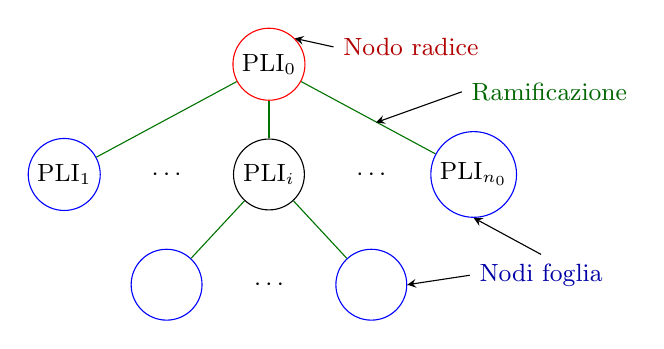
\begin{tikzpicture}[font=\small,>=stealth,
  bbnode/.style={draw,circle,inner sep=2pt,minimum size=9mm}]
  \node[bbnode,draw=red] (r) at (0,0) {$\BBpli{0}$};
  \node[bbnode,draw=blue] (l) at (-2.6,-1.4) {$\BBpli{1}$};
  \node[bbnode] (m) at (0,-1.4) {$\BBpli{i}$};
  \node[bbnode,draw=blue] (n) at (2.6,-1.4) {$\BBpli{n_0}$};
  \node[bbnode,draw=blue] (s) at (-1.3,-2.8) {};
  \node[bbnode,draw=blue] (t) at (1.3,-2.8) {};
  \foreach \u/\v in {r/l,r/m,r/n,m/s,m/t}
    \draw[green!45!black] (\u)--(\v);
  \foreach \x/\y in {-1.3/-1.4,1.3/-1.4,0/-2.8}
    \node at (\x,\y) {$\cdots$};
  \node[red!70!black,right] (a) at (.82,.22) {Nodo radice};
  \draw[->] (a.west)--(r.north east);
  \node[green!40!black,right] (b) at (2.45,-.35) {Ramificazione};
  \draw[->] (b.west)--(1.36,-.74);
  \node[blue!65!black,right] (c) at (2.55,-2.68) {Nodi foglia};
  \draw[->] (c.west)--(t.east);
  \draw[->] (c.north)--(n.south);
\end{tikzpicture}
\BBfig{3.12}{Radice, ramificazioni e foglie di un albero delle decisioni.}
\end{center}

\subsubsection{Rilassamento continuo e costruzione dei figli}

\begin{definition}{Rilassamento continuo di un nodo}
Dato $\BBpli{t}$, si ottiene $\BBrel{t}$ consentendo alle variabili intere
di assumere valori reali e conservando tutti i vincoli lineari del nodo.
Si indicano con $P_t$ la regione così ottenuta e con $X_t$ la regione
intera. Per la PLI pura qui considerata vale $X_t=P_t\cap\mathbb Z^n$.
\end{definition}

Il rilassamento continuo è la tecnica di rilassamento utilizzata nelle
dispense per decidere come partizionare il nodo. Alla radice si risolve
\[
 (\BBrel{0})\qquad \min\{c^\top x:Ax\approx b,\ x\in\mathbb R^n_{\geq 0}\}.
\]
Sia $x^*_{P_0}$ una soluzione ottima finita. Se tutte le componenti
sono intere, questa soluzione risolve anche $\BBpli{0}$. Altrimenti si
sceglie una componente frazionaria $[x^*_{P_0}]_h=a\notin\mathbb Z$.

\begin{definition}{Variabile e vincoli di branching}
La variabile $x_h$ scelta per ramificare è la \emph{variabile di branching}.
I due \emph{vincoli di branching} sono $x_h\leq\lfloor a\rfloor$ e
$x_h\geq\lceil a\rceil$, dove $\lfloor a\rfloor$ è il massimo intero
minore o uguale ad $a$ e $\lceil a\rceil$ il minimo intero maggiore o
uguale ad $a$. Ciascun figlio eredita i vincoli del padre e riceve uno
solo dei due nuovi vincoli.
\end{definition}

\[
\begin{aligned}
 (\BBpli{1})\quad &\min\{c^\top x:Ax\approx b,\ x_h\leq\lfloor a\rfloor,\
                          x\in\mathbb Z^n_{\geq0}\},\\
 (\BBpli{2})\quad &\min\{c^\top x:Ax\approx b,\ x_h\geq\lceil a\rceil,\
                          x\in\mathbb Z^n_{\geq0}\}.
\end{aligned}
\]
Poiché $a$ è frazionario, $\lceil a\rceil=\lfloor a\rfloor+1$.
Le due alternative coprono perciò tutti i valori interi di $x_h$ e sono
incompatibili. Nei rilassamenti, invece, si elimina la striscia aperta
$\lfloor a\rfloor<x_h<\lceil a\rceil$, che contiene la soluzione
continua del padre.

\begin{center}
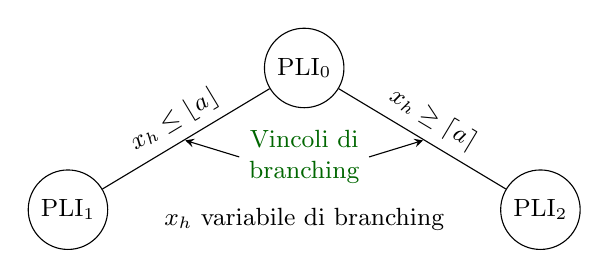
\begin{tikzpicture}[font=\small,>=stealth,
  bbnode/.style={draw,circle,inner sep=3pt}]
  \node[bbnode] (r) at (0,0) {$\BBpli{0}$};
  \node[bbnode] (l) at (-3,-1.8) {$\BBpli{1}$};
  \node[bbnode] (d) at (3,-1.8) {$\BBpli{2}$};
  \draw (r)--node[above,sloped] {$x_h\leq\lfloor a\rfloor$} (l);
  \draw (r)--node[above,sloped] {$x_h\geq\lceil a\rceil$} (d);
  \node[align=center,green!40!black] (b) at (0,-1.13) {Vincoli di\\branching};
  \draw[->] (b.west)--(-1.51,-.92);
  \draw[->] (b.east)--(1.51,-.92);
  \node at (0,-1.92) {$x_h$ variabile di branching};
\end{tikzpicture}
\BBfig{3.13}{Ramificazione quando $[x^*_{P_0}]_h=a\notin\mathbb Z$.}
\end{center}

Per ogni figlio si risolve il corrispondente rilassamento continuo e,
se necessario, si ripete la ramificazione. In un generico nodo $t$ si
ritrovano i vincoli originari $Ax\approx b$, $x\geq0$ e tutti i vincoli
di branching incontrati sull'unico cammino dalla radice a $t$.
Il vincolo di integralità caratterizza il problema intero di ciascun nodo.
Una discesa nell'albero restringe l'insieme delle soluzioni candidate.
In linea di principio si potrebbero enumerare tutte le soluzioni intere.
Le condizioni di chiusura consentono di evitare l'esplorazione esplicita
di molti nodi.

\subsection{Criterio di bounding}

\begin{definition}{Migliore soluzione nota e limite del rilassamento}
La migliore soluzione intera ammissibile trovata finora per il problema
originario è detta \emph{incumbent} e si indica con $\BBsol$.
Il suo valore è $\BBinc=z(\BBsol)$. In assenza di una soluzione iniziale,
si pone simbolicamente $\BBsol=\varnothing$, con $\BBinc=+\infty$ nel
minimo e $\BBinc=-\infty$ nel massimo. Se è già disponibile una soluzione
ammissibile, si inizializzano entrambi con quella soluzione e il suo valore.
Il valore ottimo del rilassamento al nodo $t$ fornisce un limite inferiore
nel minimo e un limite superiore nel massimo.
\end{definition}

Siano $P_t^*$ e $X_t^*$ gli insiemi delle soluzioni ottime rispettivamente
del rilassamento e del problema intero. Le relazioni richiamate nella nota
delle pp.~111--112 si giustificano con l'inclusione $X_t\subseteq P_t$.
\begin{enumerate}
 \item Se $P_t=\varnothing$, anche $X_t=\varnothing$, perché una soluzione
       intera ammissibile sarebbe pure ammissibile per il rilassamento.
 \item Se l'obiettivo del problema intero è illimitato nella direzione
       di ottimizzazione, anche quello del rilassamento è illimitato
       nella stessa direzione. Infatti la stessa successione di soluzioni
       è ammissibile in $P_t$. Nella notazione delle dispense l'implicazione
       di illimitatezza è scritta $z^*_{\BBpli{t}}=\infty\Rightarrow
       z^*_{\BBrel{t}}=\infty$. Con il segno esplicito si usa $-\infty$
       per un minimo illimitato inferiormente e $+\infty$ per un massimo
       illimitato superiormente. L'inammissibilità è trattata al punto 1.
 \item Se entrambi gli ottimi esistono, nel minimo
       $z^*_{\BBrel{t}}\leq z^*_{\BBpli{t}}$. Il rilassamento può infatti
       scegliere anche la soluzione ottima intera. Nel massimo si ottiene
       $z^*_{\BBrel{t}}\geq z^*_{\BBpli{t}}$.
 \item Se $y\in P_t^*\cap\mathbb Z^n$, allora $y\in X_t^*$ e
       $z(y)=z^*_{\BBrel{t}}=z^*_{\BBpli{t}}$. Infatti $y$ è ammissibile
       per il problema intero e nessun punto di $X_t\subseteq P_t$ può
       avere valore migliore di $y$.
\end{enumerate}

\subsubsection{Le tre condizioni di chiusura}

\begin{enumerate}
 \item \textbf{Inammissibilità.} Se il sistema dei vincoli originari
 e dei vincoli ereditati lungo il cammino fino a $t$ è incompatibile,
 $P_t=\varnothing$. Né il nodo né alcun discendente contiene una soluzione
 intera ammissibile.
 \item \textbf{Ottimo continuo intero.} Se una soluzione ottima
 $x^*_{P_t}$ è intera, è ottima anche per $\BBpli{t}$. Se migliora
 l'incumbent, si aggiornano $\BBsol\gets x^*_{P_t}$ e
 $\BBinc\gets z(x^*_{P_t})$. Il nodo è risolto anche quando il suo
 valore non migliora l'incumbent.
 \item \textbf{Bounding.} Anche con una soluzione ottima frazionaria si
 chiude $t$ quando il limite del rilassamento dimostra che nessun
 discendente può migliorare $\BBinc$.
\end{enumerate}

\emph{Giustificazione del criterio di bounding.}
Nel minimo, se $x^*_{X_t}$ è una migliore soluzione intera ottenibile
sotto $t$, si ha $c^\top x^*_{P_t}\leq c^\top x^*_{X_t}$.
Per ogni punto intero $y$ di qualunque discendente, $y\in X_t\subseteq P_t$.
Dunque, se il rilassamento ha già valore maggiore o uguale a quello
dell'incumbent,
\[
 \BBinc\leq c^\top x^*_{P_t}\leq c^\top y.
\]
Nel massimo tutti i versi si invertono. Si ha
$c^\top x^*_{P_t}\geq c^\top x^*_{X_t}$ e si può chiudere il nodo se
\[
 c^\top y\leq c^\top x^*_{P_t}\leq\BBinc.
\]
L'uguaglianza basta se si cerca una soluzione ottima. Un altro punto
dello stesso valore non migliorerebbe il risultato.

\subsection{Scelta della variabile di branching}

Si consideri un nodo $t$ con ottimo continuo frazionario per il quale
non è verificato il criterio di bounding. Gli indici tra cui scegliere sono
\[
 F=\{\ell\in\{1,\dots,n\}:[x^*_{P_t}]_\ell\notin\mathbb Z\}.
\]
Se $|F|=1$ la scelta è obbligata. Se $|F|\geq2$, le dispense indicano
tre criteri corretti, senza attribuire a uno di essi una superiorità generale.
\begin{enumerate}
 \item Scegliere casualmente $h\in F$.
 \item Scegliere il minimo indice, ossia $h=\min F$.
 \item Scegliere un indice al quale la componente frazionaria assume il
       valore più piccolo,
       $h\in\operatorname*{arg\,min}_{\ell\in F}[x^*_{P_t}]_\ell$.
       Il minimo è calcolato sui valori delle componenti in $F$, come
       nella formula delle dispense. L'operatore $\arg\min$ restituisce
       gli indici che realizzano quel minimo.
\end{enumerate}

\subsection{Branch \& Bound: esempio numerico}

Si consideri il problema di massimo con funzione obiettivo
$z(x)=x_1+3x_2$. Per mantenere visibili i vincoli ereditati, si scriverà
esplicitamente il modello di ciascun nodo.

\newcommand{\BBmodello}[3]{%
 \[
 \begin{aligned}
 (#1)\qquad \max\quad &x_1+3x_2\\
 \text{soggetto a}\quad &x_1\geq\tfrac12 &&(a)\\
 &x_1+\tfrac75x_2\leq\tfrac{13}{2} &&(b)\\
 &-5x_1+3x_2\leq5 &&(c)\\
 #2
 &(x_1,x_2)\in #3.
 \end{aligned}
 \]}
\newcommand{\BBdestra}{&x_1\geq2 &&(d')\\}
\newcommand{\BBbasso}{&x_2\leq3 &&(e)\\}

\BBmodello{\BBpli{0}}{}{\mathbb Z_{\geq0}^2}

La regione intera è $X_0$ e il valore cercato è $z^*_{\BBpli{0}}$.
Si inizializza $\BBsol=\varnothing$, $\BBinc=-\infty$.

\subsubsection{Radice e ottimo del rilassamento}

\BBmodello{\BBrel{0}}{}{\mathbb R_{\geq0}^2}

Per costruire il poligono $P_0$ si riscrivono i vincoli obliqui come
\[
 (b)\quad x_2\leq\frac{65}{14}-\frac57x_1,
 \qquad
 (c)\quad x_2\leq\frac53+\frac53x_1.
\]
Il vertice $A$ è l'intersezione delle due rette. Sostituendo l'uguaglianza
di $(c)$ in $(b)$ si ottiene
\[
 x_1+\frac75\left(\frac53+\frac53x_1\right)=\frac{13}{2},
 \quad 6x_1+14+14x_1=39,
 \quad 20x_1=25,
 \quad x_1=\frac54.
\]
Quindi $x_2=\tfrac53(1+\tfrac54)=\tfrac{15}{4}$.
Per $B$, da $(a)$ all'uguaglianza si ricava $x_1=1/2$, e da $(c)$
$x_2=\tfrac53(1+\tfrac12)=\tfrac52$. Sull'asse $x_2=0$ i vincoli
$(a)$ e $(b)$ danno rispettivamente $C=(1/2,0)$ e $D=(13/2,0)$.
Poiché una funzione lineare su questo poligono raggiunge il massimo in
un vertice, basta confrontare i quattro valori.

\begin{center}
\begin{tabular}{c c l}
\hline
Vertice & $(x_1,x_2)$ & $z=x_1+3x_2$\\
\hline
$A$ & $(5/4,15/4)$ & $5/4+45/4=50/4$\\
$B$ & $(1/2,5/2)$   & $1/2+15/2=8$\\
$C$ & $(1/2,0)$     & $1/2+0=1/2$\\
$D$ & $(13/2,0)$    & $13/2+0=13/2$\\
\hline
\end{tabular}
\end{center}

Segue $x^*_{P_0}=A=(5/4,15/4)$ e $z^*_{\BBrel{0}}=50/4$.
Entrambe le componenti sono frazionarie. Si sceglie $x_1$ per la prima
ramificazione.

\newcommand{\BBpunto}[3]{%
 \fill[#3] (#1) rectangle ++(.055,.055);
 \node[#2,text=#3,inner sep=1pt] at (#1) {$#1$};}

\newcommand{\BBgrafico}[3]{%
\begin{center}
\begin{tikzpicture}[x=1.02cm,y=.90cm,>=stealth,font=\scriptsize,
 base/.style={brown!65!black,thick},verso/.style={brown!65!black,->}]
 \coordinate (A) at (1.25,3.75); \coordinate (B) at (.5,2.5);
 \coordinate (C) at (.5,0);       \coordinate (D) at (6.5,0);
 \coordinate (E) at (1,{10/3});   \coordinate (F) at (1,0);
 \coordinate (G) at (2,0);        \coordinate (H) at (2,{45/14});
 \coordinate (J) at (2.3,3);      \coordinate (K) at (2,3);
 \coordinate (L) at (3,2.5);      \coordinate (M) at (3,0);
 \draw[->] (-.48,0)--(7.08,0) node[below] {$x_1$};
 \draw[->] (0,-.30)--(0,5.72) node[left] {$x_2$};
 \foreach \i in {1,...,6}
   \draw (\i,.04)--(\i,-.05) node[below=1pt] {$\i$};
 \foreach \j in {1,...,4}
   \draw (.04,\j)--(-.05,\j) node[left=1pt] {$\j$};
 \draw[base] (.5,-.19)--(.5,5.20) node[above] {$(a)$};
 \draw[verso] (.5,4.88)--(.85,4.88);
 \draw[base] (-.48,{65/14+(.48)*5/7}) node[above left] {$(b)$}
   --(6.76,{65/14-6.76*5/7});
 \draw[verso] (-.35,{65/14+.35*5/7})--(-.59,4.51);
 \draw[base] (-.96,{(1-.96)*5/3})--(1.84,{(1+1.84)*5/3})
   node[above left] {$(c)$};
 \draw[verso] (1.69,{(1+1.69)*5/3})--(1.97,4.30);
 \draw[base] (-.99,1.00)--(2.72,-.237);
 \draw[verso] (-.76,.923)--(-.59,1.43);
 \node[below left] at (-.65,.84) {f.o.};
 \ifnum#1=1
   \draw[base] (1,-.18)--(1,5.35) node[above] {$(d)$};
   \draw[verso] (1,5.12)--(.68,5.12);
 \fi
 \ifnum#1>1
   \draw[base] (2,-.18)--(2,5.35) node[above right] {$(d')$};
   \draw[verso] (2,5.14)--(2.36,5.14);
 \fi
 \ifnum#1>2
   \ifnum#1=4
     \draw[base] (-.42,4)--(6.35,4) node[right] {$(e')$};
     \draw[verso] (6.02,4)--(6.02,4.37);
   \else
     \draw[base] (-.42,3)--(6.35,3) node[right] {$(e)$};
     \draw[verso] (6.02,3)--(6.02,2.65);
   \fi
 \fi
 \ifnum#1=5
   \node[above left] at (1.91,5.35) {$(f)$};
   \draw[verso] (2,5.14)--(1.63,5.14);
   \draw[very thick] (G)--(K);
 \fi
 \ifnum#1=6
   \draw[base] (3,-.18)--(3,5.35) node[above] {$(f')$};
   \draw[verso] (3,5.14)--(3.36,5.14);
   \node[left] at (-.45,3) {$(e)$};
 \fi
 \BBpunto{B}{above left}{black}
 \BBpunto{C}{above left}{black}
 \BBpunto{D}{above right}{red!70!black}
 \ifnum#1<3
   \fill[red!70!black] (A) circle (1.4pt);
   \ifnum#1=0
     \node[above right,red!70!black] at (A) {$A=x^*_{P_0}=(5/4,15/4)$};
   \else
     \node[above right,red!70!black] at (A) {$A=(5/4,15/4)$};
   \fi
 \else
   \BBpunto{A}{above left}{black}
 \fi
 \ifnum#1=1
   \BBpunto{E}{above left}{red!70!black}
   \BBpunto{F}{above left}{red!70!black}
 \fi
 \ifnum#1>1
   \BBpunto{G}{above left}{red!70!black}
   \fill[red!70!black] (H) circle (1.2pt);
   \ifnum#1<5
     \ifnum#1=2
       \node[above right] at (H) {$H$};
     \else
       \node[above right,red!70!black] at (H) {$H=(2,45/14)$};
     \fi
   \else
     \node[above right] at (H) {$H$};
   \fi
 \fi
 \ifnum#1>2
   \ifnum#1=4\else
     \BBpunto{K}{below left}{red!70!black}
     \fill[red!70!black] (J) circle (1.2pt);
     \ifnum#1=3
       \node[below right] at (J) {$J$};
     \else
       \node[above right,red!70!black] at (J) {$J=(23/10,3)$};
     \fi
   \fi
 \fi
 \ifnum#1=6
   \BBpunto{L}{below left}{red!70!black}
   \BBpunto{M}{above left}{red!70!black}
 \fi
 \ifcase#1
   \node at (2.72,1.65) {$P_0$};
 \or \node at (.76,1.67) {$P_1$};
 \or \node at (3.64,1.05) {$P_2$};
 \or \node at (3.64,1.05) {$P_3$};
 \or \node at (3.60,4.49) {$P_4=\varnothing$};
 \or \node[rotate=-90] at (2.25,1.45) {$P_5=\overline{KG}$};
 \or \node at (4.30,.85) {$P_6$};
 \fi
\end{tikzpicture}
\BBfig{#2}{#3}
\end{center}}

\BBgrafico{0}{3.14}{Regione ammissibile $P_0$ e ottimo del rilassamento
alla radice. La freccia sulla retta di livello della f.o. indica il verso
di crescita di $x_1+3x_2$.}

\subsubsection{Prima ramificazione: da $X_0$ a $X_1$ e $X_2$}

Da $1<5/4<2$ seguono $\lfloor5/4\rfloor=1$ e $\lceil5/4\rceil=2$.
Si generano i due problemi
\BBmodello{\BBpli{1}}{&x_1\leq\lfloor5/4\rfloor=1 &&(d)\\}{\mathbb Z_{\geq0}^2}
\BBmodello{\BBpli{2}}{&x_1\geq\lceil5/4\rceil=2 &&(d')\\}{\mathbb Z_{\geq0}^2}

I rilassamenti si ottengono sostituendo $\mathbb R_{\geq0}^2$ a
$\mathbb Z_{\geq0}^2$. Per le regioni vale
\[
 X_1\cup X_2=X_0,\quad X_1\cap X_2=\varnothing,\qquad
 P_1\cup P_2\subsetneq P_0,\quad P_1\cap P_2=\varnothing.
\]
L'inclusione è stretta perché, ad esempio, $A$ appartiene a $P_0$ ma
non appartiene a nessuno dei due rilassamenti figli.

\paragraph{Nodo 1.}
Nel tratto $1/2\leq x_1\leq1$ il bordo superiore è dato da $(c)$.
Su questo bordo
\[
 x_2=\frac{5+5x_1}{3},\qquad
 z=x_1+3\frac{5+5x_1}{3}=5+6x_1.
\]
Il valore cresce con $x_1$. All'estremo $x_1=1$ si trova
$E=(1,10/3)$, mentre sul bordo inferiore si ha $F=(1,0)$.
I vertici $C,B,E,F$ danno rispettivamente $1/2,8,11,1$. Pertanto
\[
 x^*_{P_1}=E=\left(1,\frac{10}{3}\right)\notin\mathbb Z^2,
 \qquad z^*_{\BBrel{1}}=1+3\frac{10}{3}=11.
\]
\BBgrafico{1}{3.15}{Regione $P_1$ del rilassamento del nodo 1.}

\paragraph{Nodo 2.}
Per $x_1\geq2$ il bordo superiore è dato da $(b)$. Su questo bordo
\[
 z=x_1+3\left(\frac{65}{14}-\frac57x_1\right)
   =\frac{195}{14}-\frac87x_1.
\]
Il coefficiente di $x_1$ è negativo, quindi il massimo si ottiene per
$x_1=2$. Sostituendo in $(b)$ si ricava
\[
 x_2=\left(\frac{13}{2}-2\right)\frac57
     =\frac92\frac57=\frac{45}{14}.
\]
I vertici del triangolo sono $G=(2,0)$, $D=(13/2,0)$ e
$H=(2,45/14)$, con valori $2$, $13/2$ e
\[
 z^*_{\BBrel{2}}=z(H)=2+3\frac{45}{14}
   =\frac{28+135}{14}=\frac{163}{14}.
\]
Anche $x^*_{P_2}=H$ è frazionario. Finora nessun rilassamento ha fornito
una soluzione ottima intera. I nodi 1 e 2 restano da valutare ulteriormente.
\BBgrafico{2}{3.16}{Regione $P_2$ del rilassamento del nodo 2.}

\newcommand{\BBalbero}[3]{%
\begin{center}
\begin{tikzpicture}[x=1cm,y=1cm,font=\scriptsize,
 n/.style={circle,draw,minimum size=8mm,inner sep=1.5pt}]
 \node[n] (r) at (0,0) {$\BBpli{0}$};
 \node[n] (a) at (-2,-1.6) {$\BBpli{1}$};
 \node[n] (b) at (2,-1.6) {$\BBpli{2}$};
 \draw (r)--node[above left] {$x_1\leq1$} (a);
 \draw (r)--node[above right] {$x_1\geq2$} (b);
 \ifnum#1<3
   \node[above right,align=left] at (.28,.18)
      {$\BBinc=-\infty$\\$\BBsol=\varnothing$};
   \node[left] at (a.west) {$z(x^*_{P_1})=11$};
 \else
   \node[left,align=right] at (a.west) {$z(x^*_{P_1})=11$\\$=\BBinc$};
 \fi
 \node[right] at (b.east) {$z(x^*_{P_2})=163/14$};
 \ifnum#1>1
   \node[n] (c) at (0,-3.2) {$\BBpli{3}$};
   \node[n] (d) at (4,-3.2) {$\BBpli{4}$};
   \draw (b)--node[above left] {$x_2\leq3$} (c);
   \draw (b)--node[above right] {$x_2\geq4$} (d);
   \node[left] at (c.west) {$z(x^*_{P_3})=113/10$};
   \draw[double] (3.64,-3.72)--(4.36,-3.72);
 \fi
 \ifnum#1=3
   \node[n] (e) at (-2,-4.8) {$\BBpli{5}$};
   \node[n] (f) at (2,-4.8) {$\BBpli{6}$};
   \draw (c)--node[above left] {$x_1\leq2$} (e);
   \draw (c)--node[above right] {$x_1\geq3$} (f);
   \node[left,align=right,red!65!black] at (e.west)
     {$\BBsol=x^*_{P_5}=(2,3)$\\$\BBinc=z(x^*_{P_5})=11$};
   \node[right,align=left] at (f.east)
     {$z(x^*_{P_6})=21/2$\\$<\BBinc$};
   \draw[double] (-2.36,-2.12)--(-1.64,-2.12);
   \draw[double] (-2.36,-5.32)--(-1.64,-5.32);
   \draw[double] (1.64,-5.32)--(2.36,-5.32);
 \fi
\end{tikzpicture}
\BBfig{#2}{#3}
\end{center}}

\BBalbero{1}{3.17}{Prima operazione di branching. I valori accanto ai
figli sono limiti superiori.}

\subsubsection{Seconda ramificazione: da $X_2$ a $X_3$ e $X_4$}

Si sceglie il nodo 2. In $H=(2,45/14)$ la sola componente frazionaria è
$x_2$. Poiché $42/14<45/14<56/14$, si ha
$\lfloor45/14\rfloor=3$ e $\lceil45/14\rceil=4$. Entrambi i figli
ereditano $x_1\geq2$.

\BBmodello{\BBpli{3}}{\BBdestra
 &x_2\leq\lfloor45/14\rfloor=3 &&(e)\\}{\mathbb Z_{\geq0}^2}
\BBmodello{\BBpli{4}}{\BBdestra
 &x_2\geq\lceil45/14\rceil=4 &&(e')\\}{\mathbb Z_{\geq0}^2}

\paragraph{Nodo 3.}
La retta $x_2=3$ incontra $x_1=2$ in $K=(2,3)$ e la retta $(b)$ in $J$.
La prima coordinata di $J$ si calcola da
\[
 x_1+\frac75\cdot3=\frac{13}{2}
 \quad\Longrightarrow\quad
 x_1=\frac{13}{2}-\frac{21}{5}=\frac{65-42}{10}=\frac{23}{10}.
\]
Il quadrilatero ha vertici $G,K,J,D$. Confrontando i valori
\[
 z(G)=2,\quad z(K)=2+9=11,\quad
 z(J)=\frac{23}{10}+9=\frac{113}{10},\quad z(D)=\frac{13}{2},
\]
si trova $x^*_{P_3}=J=(23/10,3)\notin\mathbb Z^2$ e
$z^*_{\BBrel{3}}=113/10$. Nell'esecuzione illustrata si aggiorna
l'incumbent quando si incontra un ottimo continuo intero. Il vertice $K$
sarà registrato al nodo 5.
\BBgrafico{3}{3.18}{Regione $P_3$ dopo l'aggiunta di $x_2\leq3$.}

\paragraph{Nodo 4.}
Da $x_1\geq2$ e $x_2\geq4$ seguirebbe
\[
 x_1+\frac75x_2\geq2+\frac{28}{5}=\frac{38}{5}
  =\frac{76}{10}>\frac{65}{10}=\frac{13}{2},
\]
in contraddizione con $(b)$. Quindi $P_4=\varnothing$ e anche
$X_4=\varnothing$. Si chiude il nodo per inammissibilità. Restano i nodi
1 e 3, con $\BBinc=-\infty$.
\BBgrafico{4}{3.19}{Il sistema che definisce $P_4$ è incompatibile.}
\BBalbero{2}{3.20}{Seconda operazione di branching. La doppia linea
sotto il nodo 4 ne indica la chiusura.}

\subsubsection{Terza ramificazione: da $X_3$ a $X_5$ e $X_6$}

Si sceglie il nodo 3. Nel punto $J=(23/10,3)$ è frazionaria $x_1$.
Da $2<23/10<3$ seguono i vincoli $x_1\leq2$ e $x_1\geq3$.
Rimangono in entrambi i figli $x_1\geq2$ e $x_2\leq3$, ereditati
dal cammino precedente.

\BBmodello{\BBpli{5}}{\BBdestra\BBbasso
 &x_1\leq\lfloor23/10\rfloor=2 &&(f)\\}{\mathbb Z_{\geq0}^2}
\BBmodello{\BBpli{6}}{\BBdestra\BBbasso
 &x_1\geq\lceil23/10\rceil=3 &&(f')\\}{\mathbb Z_{\geq0}^2}

\paragraph{Nodo 5.}
I vincoli $(d')$ e $(f)$ impongono insieme $x_1=2$. Per tale valore
$(b)$ dà $x_2\leq45/14$, $(c)$ dà $3x_2\leq15$, ossia $x_2\leq5$,
e $(e)$ impone $x_2\leq3$. Poiché $3<45/14<5$, risulta
\[
 P_5=\{(2,x_2):0\leq x_2\leq3\}=\overline{KG}.
\]
Sul segmento l'obiettivo è $2+3x_2$, crescente. In $G$ vale $2$ e in
$K$ vale $2+3\cdot3=11$. Pertanto
\[
 x^*_{P_5}=K=(2,3)\in\mathbb Z^2,\qquad
 z^*_{\BBrel{5}}=z^*_{\BBpli{5}}=11.
\]
Il nodo si chiude per integralità. Si aggiornano
$\BBsol\gets(2,3)$ e $\BBinc\gets11$.
\BBgrafico{5}{3.21}{La regione $P_5$ coincide con il segmento $KG$.}

\paragraph{Nodo 6.}
Il vincolo $x_1\geq3$ individua il triangolo di vertici
$M=(3,0)$, $D=(13/2,0)$ e $L$, intersezione di $x_1=3$ con $(b)$.
Si ricava
\[
 x_2=\left(\frac{13}{2}-3\right)\frac57
     =\frac72\frac57=\frac52,
 \qquad L=\left(3,\frac52\right).
\]
Si ha $z(M)=3$, $z(D)=13/2$ e
\[
 z(L)=3+3\frac52=\frac{6+15}{2}=\frac{21}{2}.
\]
Il massimo continuo è quindi raggiunto in un punto frazionario, ma ogni
soluzione intera del nodo ha valore al più $21/2<11=\BBinc$. Si chiude
il nodo per bounding.
\BBgrafico{6}{3.22}{Regione $P_6$ e ottimo continuo $L$.}

\paragraph{Ritorno al nodo 1 e certificato di ottimalità.}
Il limite già calcolato al nodo 1 è ancora valido. Il suo confronto con
l'incumbent aggiornato dà
\[
 z^*_{\BBrel{1}}=z(E)=1+3\frac{10}{3}=11\leq\BBinc=11.
\]
Si chiude quindi anche il nodo 1 per bounding, questa volta in uguaglianza.
Non rimangono sottoproblemi da investigare. Si conclude che
\[
 \boxed{x^*_{\BBpli{0}}=\BBsol=x^*_{\BBpli{5}}=x^*_{P_5}=(2,3)},
 \qquad
 \boxed{z^*_{\BBpli{0}}=\BBinc=z(x^*_{P_5})=11}.
\]
\BBalbero{3}{3.23}{Terza operazione di branching. Le foglie 1 e 6 sono
chiuse per bounding, la 4 per inammissibilità e la 5 per integralità.}

\subsection{Generazione e visita dell'albero di branching}

La scelta della variabile determina come dividere un nodo. La scelta del
prossimo nodo da esplorare stabilisce invece l'ordine di visita dell'albero.

\begin{definition}{Nodo attivo}
Un nodo attivo è un sottoproblema già generato che richiede ancora
esplorazione. Si indica con $Q$ l'insieme dei nodi attivi. L'algoritmo
termina quando $Q=\varnothing$ e anche l'elaborazione del nodo corrente
è conclusa.
\end{definition}

\subsubsection{Visita in profondità: depth first}

\begin{definition}{Depth first e backtracking}
La visita \emph{depth first} genera o visita il primo figlio di un nodo
ramificabile e prosegue ricorsivamente lungo il ramo così scelto. Ogni
discesa è un \emph{forward step}. Quando si verifica una delle tre
condizioni di chiusura, si risale al padre per esaminare un eventuale
figlio ancora da generare. La risalita prende il nome di \emph{backtracking}.
\end{definition}

Per un problema di massimo le operazioni sono le seguenti.
\begin{enumerate}
 \item Calcolare il limite superiore $U_0=z^*_{\BBrel{0}}$ alla radice.
 \item Se si deve ramificare, generare il primo figlio $\BBpli{1}$ e
       calcolare $U_1=z^*_{\BBrel{1}}$.
 \item Proseguire dall'ultimo nodo generato con una sequenza di passi
       avanti, fino a incontrare un nodo $\BBpli{k}$ da chiudere.
       Se la chiusura fornisce una soluzione intera migliore,
       aggiornare $\BBsol$ e $\BBinc$.
 \item Risalire al padre, indicato con $\BBpli{k-1}$ lungo questa
       sequenza di discese. Se $U_{k-1}>\BBinc$ ed esiste un figlio
       ancora inesplorato, generarlo come nuovo nodo $\BBpli{k+1}$ e
       riprendere la discesa. Se $U_{k-1}\leq\BBinc$ o i figli sono
       esauriti, risalire ancora al predecessore $\BBpli{k-2}$ e
       ripetere il controllo.
 \item Memorizzare in una pila $Q$ i nodi o i passi di visita ancora
       pendenti. Quando si dovrebbe risalire oltre la radice la pila è
       vuota e l'esecuzione termina.
\end{enumerate}

\paragraph{Esempio di visita per un problema di massimo.}
Le lettere nella figura 3.24 danno, in ordine alfabetico, la sequenza
di generazione e visita. Si calcolano i limiti superiori dei soli nodi
effettivamente esplorati. Si riportano i valori della figura, compresa
l'incongruenza numerica discussa sotto.

\begin{center}
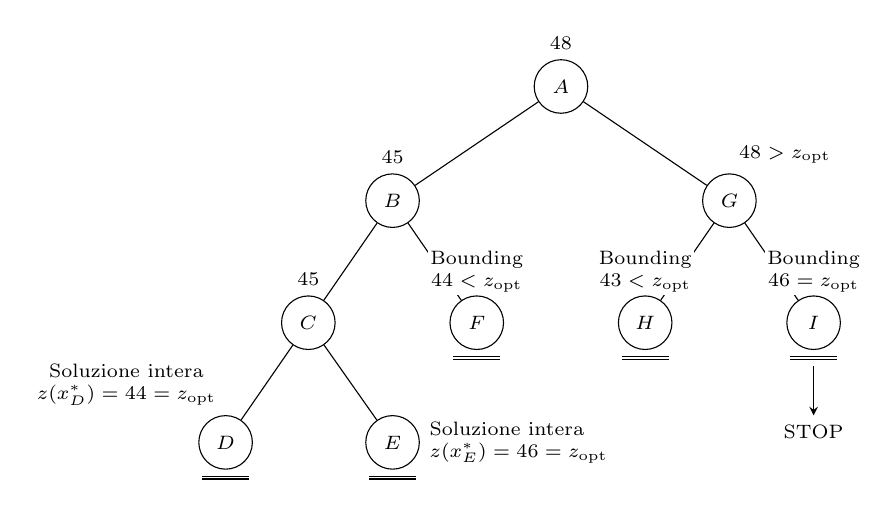
\begin{tikzpicture}[x=.93cm,y=1cm,font=\scriptsize,>=stealth,
 n/.style={circle,draw,minimum size=6.8mm,inner sep=1pt}]
 \node[n] (A) at (0,0) {$A$};
 \node[n] (B) at (-2.30,-1.45) {$B$};
 \node[n] (G) at (2.30,-1.45) {$G$};
 \node[n] (C) at (-3.45,-3) {$C$};
 \node[n] (F) at (-1.15,-3) {$F$};
 \node[n] (H) at (1.15,-3) {$H$};
 \node[n] (I) at (3.45,-3) {$I$};
 \node[n] (D) at (-4.58,-4.52) {$D$};
 \node[n] (E) at (-2.30,-4.52) {$E$};
 \foreach \u/\v in {A/B,A/G,B/C,B/F,C/D,C/E,G/H,G/I}
   \draw (\u)--(\v);
 \node[above] at (A.north) {$48$};
 \node[above] at (B.north) {$45$};
 \node[above] at (C.north) {$45$};
 \node[above right] at (G.north) {$48>\BBinc$};
 \node[above,align=center,fill=white,inner sep=1pt] at (F.north)
   {Bounding\\$44<\BBinc$};
 \node[above,align=center,fill=white,inner sep=1pt] at (H.north)
   {Bounding\\$43<\BBinc$};
 \node[above,align=center,fill=white,inner sep=1pt] at (I.north)
   {Bounding\\$46=\BBinc$};
 \node[above left,align=center] at (D.north)
   {Soluzione intera\\$z(x_D^*)=44=\BBinc$};
 \node[right,align=left] at (E.east)
   {Soluzione intera\\$z(x_E^*)=46=\BBinc$};
 \foreach \v in {D,E,F,H,I}
   \draw[double] ([xshift=-3mm,yshift=-1mm]\v.south)--
                 ([xshift=3mm,yshift=-1mm]\v.south);
 \draw[->] ([yshift=-2mm]I.south)--++(0,-.63) node[below] {STOP};
\end{tikzpicture}
\BBfig{3.24}{Visita in profondità nell'ordine $A,B,C,D,E,F,G,H,I$.}
\end{center}

\begin{enumerate}
 \item In $A$ il limite è $48$. Si scende al primo figlio $B$, di limite
       $45$, e al suo primo figlio $C$, anch'esso di limite $45$.
 \item In $D$, primo figlio di $C$, si incontra una soluzione intera di
       valore $44$. Si pone $\BBinc=44$ e si chiude $D$.
 \item Si risale a $C$. Poiché $45>44$, si visita $E$. La figura
       attribuisce alla sua soluzione intera valore $46$. L'incumbent
       rappresentato diventa quindi $46$.
 \item Esaurito il ramo di $C$, il disegno riporta $F$, secondo figlio
       di $B$, con limite $44<46$. $F$ è contrassegnato come chiuso
       per bounding.
 \item Si torna alla radice e si visita $G$. Poiché $48>46$, il suo
       ramo può ancora migliorare l'incumbent.
 \item Il primo figlio $H$ ha limite $43<46$ e si chiude per bounding.
       Il secondo figlio $I$ ha limite $46=46$ e si chiude anch'esso.
       Nessun nodo rimane da esplorare.
\end{enumerate}

\emph{Precisazione sui dati della figura 3.24.}
Poiché $E$ discende da $C$ e da $B$, una soluzione di $E$ di valore
$46$ sarebbe ammissibile anche in entrambi gli antenati. È quindi
incompatibile con i loro limiti superiori stampati, entrambi pari a $45$.
Inoltre, applicando alla lettera il controllo al ritorno in $B$,
$45\leq46$ basterebbe già a escludere il ramo di $F$. L'albero riproduce
la sequenza delle dispense e rende visibili i passi di visita, ma i valori
stampati non possono provenire tutti dalla medesima istanza di massimo.

\paragraph{Vantaggi e svantaggi.}
La ricorsione rende semplice l'implementazione. Nella visita binaria in
profondità rimane in attesa al più un ramo fratello per livello, quindi
il numero di nodi pendenti è limitato dalla profondità dell'albero.
Raggiungendo rapidamente livelli profondi si possono trovare presto
soluzioni intere e poi migliorarle. Anche un arresto anticipato, ad esempio
per un limite di tempo, può così restituire una buona soluzione ammissibile.
Per passare a un ramo lontano, tuttavia, possono occorrere numerosi passi
di backtracking.

\subsubsection{Visita secondo il miglior limite: best bound first}

\begin{definition}{Best bound first}
Si ramifica a partire dal nodo attivo il cui rilassamento continuo
presenta il limite più favorevole. Per un massimo si sceglie il limite
superiore più alto, per un minimo il limite inferiore più basso. Tale
regola privilegia il ramo con la migliore prospettiva di miglioramento
indicata dal rilassamento.
\end{definition}

Per il problema di massimo considerato nelle dispense si procede come segue.
\begin{enumerate}
 \item Risolvere $\BBrel{0}$ e calcolare $U_0=z^*_{\BBrel{0}}$.
 \item Se la radice richiede ramificazione, generare entrambi i figli
       $\BBpli{1}$ e $\BBpli{2}$ e calcolare i limiti $U_1$ e $U_2$
       dei rilassamenti ammissibili.
 \item Applicare le condizioni di chiusura, aggiornare l'eventuale
       incumbent e mantenere in $Q$ i figli che richiedono ancora una
       ramificazione e che hanno $U_i>\BBinc$.
 \item Finché $Q\ne\varnothing$, scegliere
       \[
        t\in\operatorname*{arg\,max}_{i:\,\BBpli{i}\in Q} U_i.
       \]
       Estrarre $\BBpli{t}$, generarne i figli e valutarli con le stesse
       regole. Dopo ogni miglioramento dell'incumbent si possono eliminare
       da $Q$ tutti i nodi il cui limite è ormai al più $\BBinc$.
 \item Terminare quando $Q=\varnothing$.
\end{enumerate}

Nella formula di p.~126 che descrive $Q$ compare il segno $<$.
Per un massimo il verso coerente con il criterio di bounding dimostrato
sopra è $>$, perché $U_i\leq\BBinc$ è precisamente la condizione di
chiusura. I due figli della radice, indicati due volte con lo stesso indice
in una riga della pagina, sono $\BBpli{1}$ e $\BBpli{2}$.

Il vantaggio indicato per il best bound first è che in media vengono
generati meno nodi. Lo svantaggio è che la visita tende a rimanere ai
livelli meno profondi dell'albero, dove i problemi hanno ereditato meno
vincoli di branching.

La pagina 126 rinvia alla figura 3.25 per la visita best bound first
dello stesso esempio e alla figura 3.26 per lo pseudocodice generale
del B\&B. Entrambe le figure si trovano oltre l'intervallo qui trattato.
La valutazione della complessità dell'algoritmo è lasciata per esercizio.


